%!TEX root=document.tex

\section{Experimental Evaluation}
\label{sec:experiments}
 
In this section, we present our evaluation of
\VizRecDB using both DBMS and custom execution engines, 
on a variety of datasets.
The datasets that we evaluate \VizRecDB on are listed 
in Table~\ref{tab:datasets}.


\begin{table}[htb]
  \centering \scriptsize
  \begin{tabular}{|c|c|c|c|c|c|} \hline
  Name & Description & Size & Dims & Measures & Views \\ \hline
  SYN1 & Synthetic data & 1M & 50 & 5 & 250 \\
  & Randomly distributed, & & & & \\ 
  & varying \# distinct values & & & & \\ \hline
  SYN2 & Synthetic data & 1M & 50 & 20 & 1000 \\
  & Randomly distributed, & & & & \\ 
  & varying \# distinct values & & & & \\ \hline
  SYN3-10 & Synthetic data & 1M & 20 & 1 & 20 \\
  & Randomly distributed, & & & & \\ 
  & 10 distinct values/dim & & & & \\ \hline
  SYN3-100 & Synthetic data & 1M & 20 & 1 & 20 \\
  & Randomly distributed, & & & & \\ 
  & 100 distinct values/dim & & & & \\ \hline
  BANK  & Customer Loan dataset  & 40K & 10 & 8 & 80* \\ \hline
  DIAB  & Hospital data & 100K & 10 & 8 & 80* \\
  & about diabetic patients & & & & \\ \hline
  \end{tabular}
  \caption{Datasets used for testing}
  \label{tab:datasets} 
  \vspace{-10pt}
\end{table}



\stitle{Evaluation Goals for the DBMS-backed Execution Engine:} 
The primary metric that we focus on for the DBMS-backed execution engine
evaluation is {\em latency},
i.e., how long does \VizRecDB take to return the top-$k$ results.
For the DBMS-backed execution engine, we study the impact of the following
aspects on the metrics described above:
(a) the DBMS architecture, specifically, a row-store DBMS vs.~a column-store DBMS,
(b) the individual optimizations detailed in Section~\ref{sec:dbms_optimizations},
such as sharing of computation and parallel execution, as well as 
the bin-packing-based algorithm for aggregate grouping, and
(c) the various parameters of the dataset, such as size and number of views.

\stitle{Evaluation Goals for the Custom Execution Engine:} 
The primary metrics that we focus on for the custom execution engine
are {\em latency} and {\em accuracy}, i.e., whether \VizRecDB
actually returns the top-$k$ views or not, because
in this case, \VizRecDB may incorrectly prune a view in the top-$k$.
For the custom execution engine, we study the impact of the following
aspects on the metrics described above:
(a) our three pruning strategies, 
(b) the characteristics of real datasets. 


\stitle{Highlights:}
We now present a high-level summary of our experimental results. 
\squishlist
\item Our optimizations to \VizRecDB's DBMS-based execution engine can reduce
latency on large datasets from 500 seconds (on row stores) and 100 seconds (on column stores)
to about 10 seconds for column stores, and about 20 seconds for row stores,
allowing near-interactive response times. This is {\em particularly noteworthy given that, implicitly,
\VizRecDB is running 100s of queries on the DBMS for returning responses to a single \VizRecDB query}.

\item Overall, column stores are superior to row stores 
as a backend execution engine, while row stores benefit more from the optimizations 
that we propose. For instance, row stores benefit significantly (with reductions
of up to XXX\% on latency) from applying
bin-packing-based algorithms for aggregation, 
while column stores are not affected. 

\item The latency of response scales linearly 
with the size of the dataset and with the number of views with
the DBMS-based execution engine.

\item Our pruning strategies for the custom execution engine 
enables us to reduce \VizRecDB's latency from 20 seconds to less than 2 seconds
to return the first view, representing a {\em 10-fold reduction in latency}.
Further, these latency improvements do not impact accuracy significantly;
the utility of the views suggested to the user are very close to the utilities
of the top-$k$ views on real datasets.

\squishend
We begin with an evaluation of the DBMS-backed execution engine followed by an
evaluation of our custom engine. All experiments were run on a 
single machine with 8 GB RAM and a 16 core Intel Xeon E5530 processor. 
Unless described otherwise, all experiments were 
repeated three times and the latency measures were
averaged.

\subsection{DBMS-backed Execution Engine}
\label{sec:expts_dbms_execution_engine}

% As mentioned in Section \ref{sec:dbms_execution_engine}, our DBMS-based
% execution engine leverages the DBMS API to execute view queries directly on the
% database.
% While this approach has the advantages of reusing existing query procesing
% systems and being agnostic to the specific underlying DBMS, its limitations
% include the lack of fine grained control over sharing of table scans and lack of
% ability to prune low-utility views. 
In our first set of experiments, we investigate 
how well our DBMS-backed engine
can support a \VizRecDB-style workload.
We run all our experiments in this section on two database systems: a
row-oriented database (denoted ROW) and a
column-oriented database (denoted COL);
our goal is to identify which database is a better
candidate for \VizRecDB, and also study which optimizations
work better for row-stores vs.~column stores. 

The following experiments use synthetic datasets SYN1, SYN2, SYN3-10 and
SYN3-100 (listed in Table~\ref{tab:datasets}).
The performance on the real datasets is similar and is omitted.
Using synthetic datasets allows us to control all aspects
of the data, including size, number of dimensions and measures, 
data distribution, and number of distinct values. 
We start with an evaluation of the basic framework, i.e., 
how long do row and column stores take if each view is evaluated 
in sequence, without any optimization. 
We then study the effect of adding each optimization from Section~\ref{sec:dbms_optimizations} 
in turn.

\stitle{Basic No Optimization Framework:} 

{\em \underline{Summary:} Applying no optimizations 
leads to 100 seconds or more of latency on both row and column stores;
latency increases linearly as the size of the dataset, and the number
of views is increased. Column stores are superior to row stores,
with 1/5th the latency.}
Without any optimizations, the basic DBMS-backed execution engine
serially executes individual view queries, two for each possible view.
Figures \ref{fig:baseline_size} and \ref{fig:baseline_views} show
\VizRecDB\ latency when using the basic framework.
For these experiments, we used the SYN1 dataset and we created subsets of the dataset with
varying numbers of rows and views, by varying the number of dimension attributes. 
In Figure \ref{fig:baseline_size} we show the latency of \VizRecDB\ as a function
of the number of rows (100K rows --- 1M rows) in the dataset and in 
Figure \ref{fig:baseline_views} we show the latency as a function 
of the number of possible views (50 --- 250).
First, notice that the basic no optimization framework has very 
poor performance: the row store takes between 50-500s, 
while the column store takes 10-100s. 
This is because both row and column stores are implicitly
running between 50 to 250 view queries for a single \VizRecDB query.
These time scales are not practical for
any interactive applications. 
Second, column stores run about 5X faster than row stores. 
This is expected because individual view queries only select one dimension
attribute and one measure attribute at a time.  
The column store can just read these two
columns, whereas the row-store must read all data from each table.
Third, as expected, the latency of the
basic framework is directly proportional to the number of rows as well as the 
number of views in the table.

Since the latencies for the basic framework are very high for interactive
applications, it is clear that aggressive optimization needs to be employed. 

% \begin{figure}[h] 
% \centerline{
% \resizebox{4cm}{!} {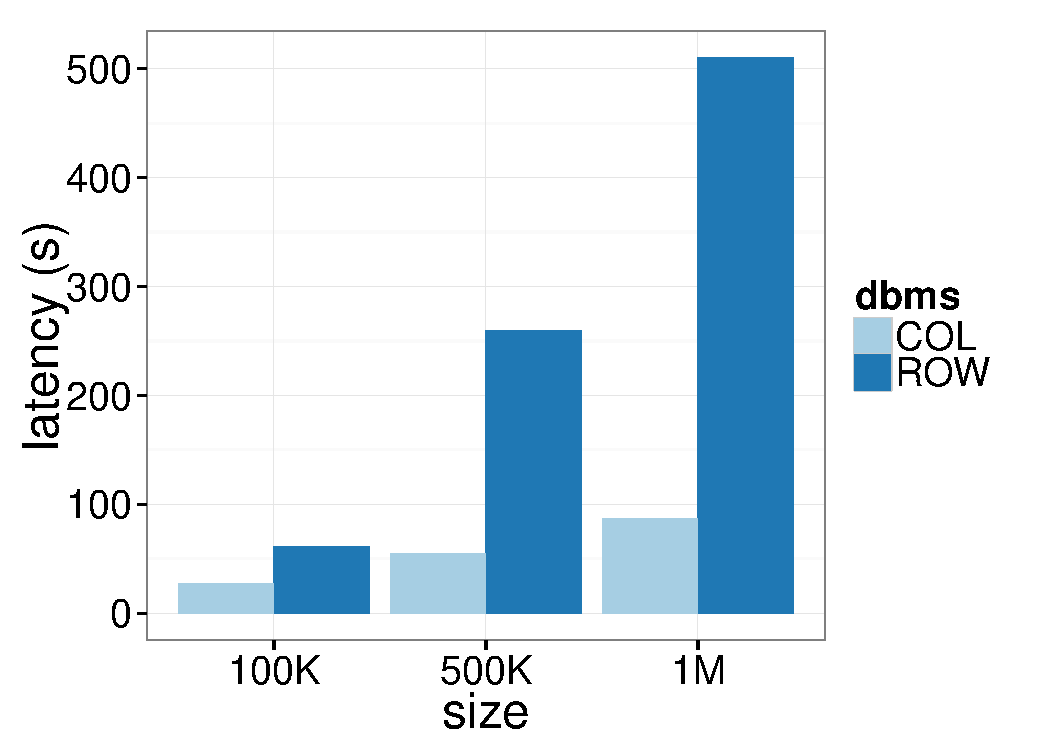
\includegraphics {Images/baselines_by_size.pdf}}
% \resizebox{4cm}{!} {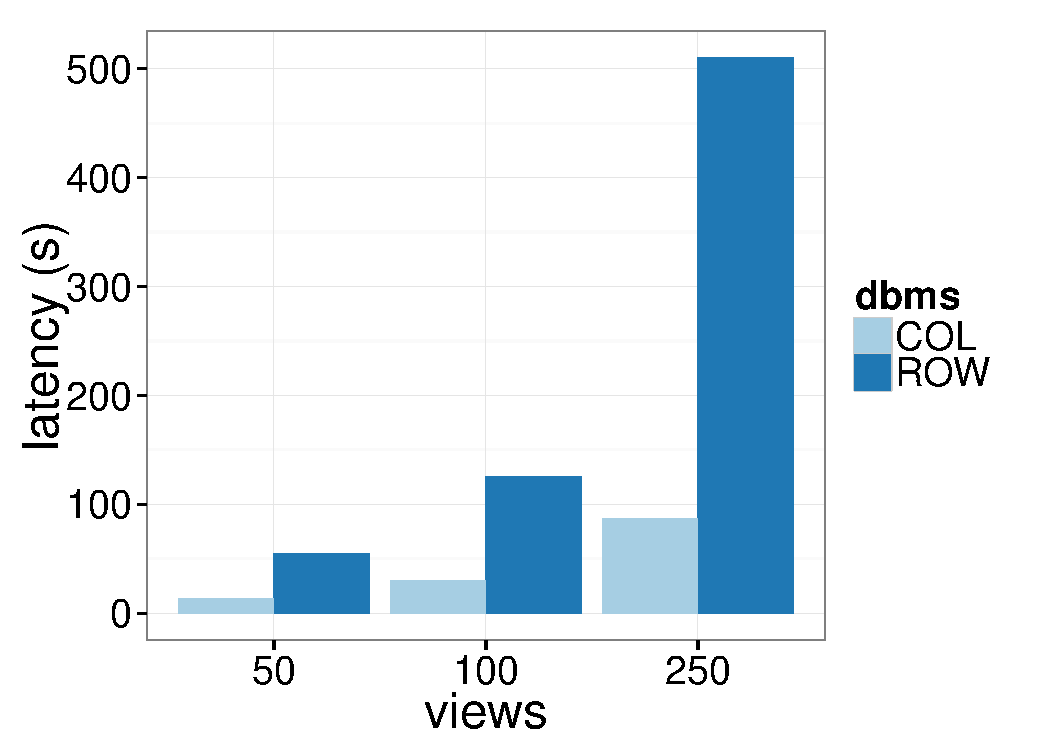
\includegraphics {Images/baselines_by_views.pdf}}
% }
% \end{figure}

\begin{figure*}[t]
	\centering
	\begin{subfigure}{0.33\linewidth}
		{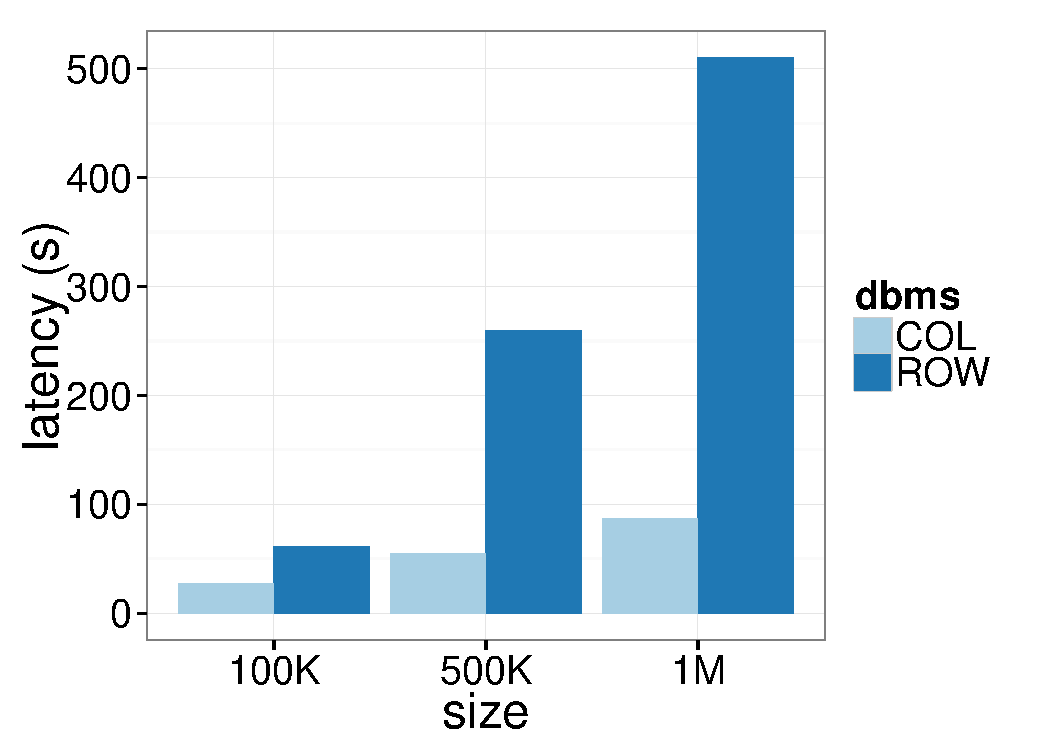
\includegraphics[width=6cm] {Images/baselines_by_size.pdf}}
		\caption{Latency vs. Table size}
		\label{fig:baseline_size}
	\end{subfigure}
	\begin{subfigure}{0.33\linewidth}
		\centering
		{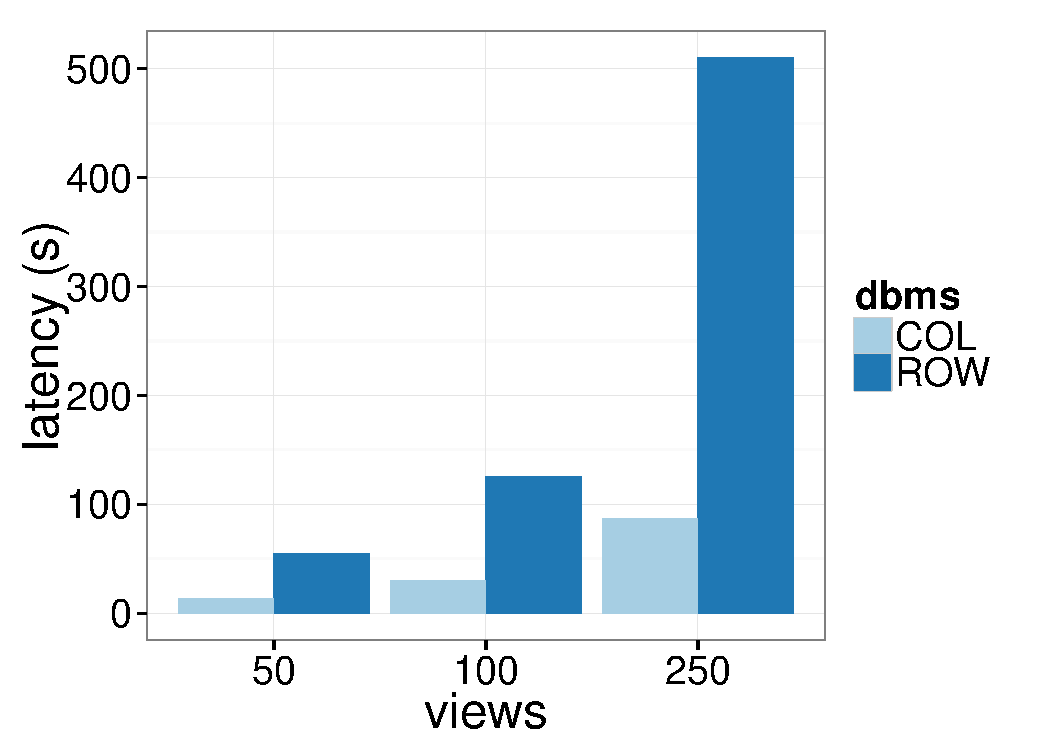
\includegraphics[width=6cm] {Images/baselines_by_views.pdf}}
		\caption{Latency vs. Num Views}
		\label{fig:baseline_views}
	\end{subfigure}
	\begin{subfigure}{0.33\linewidth}
		{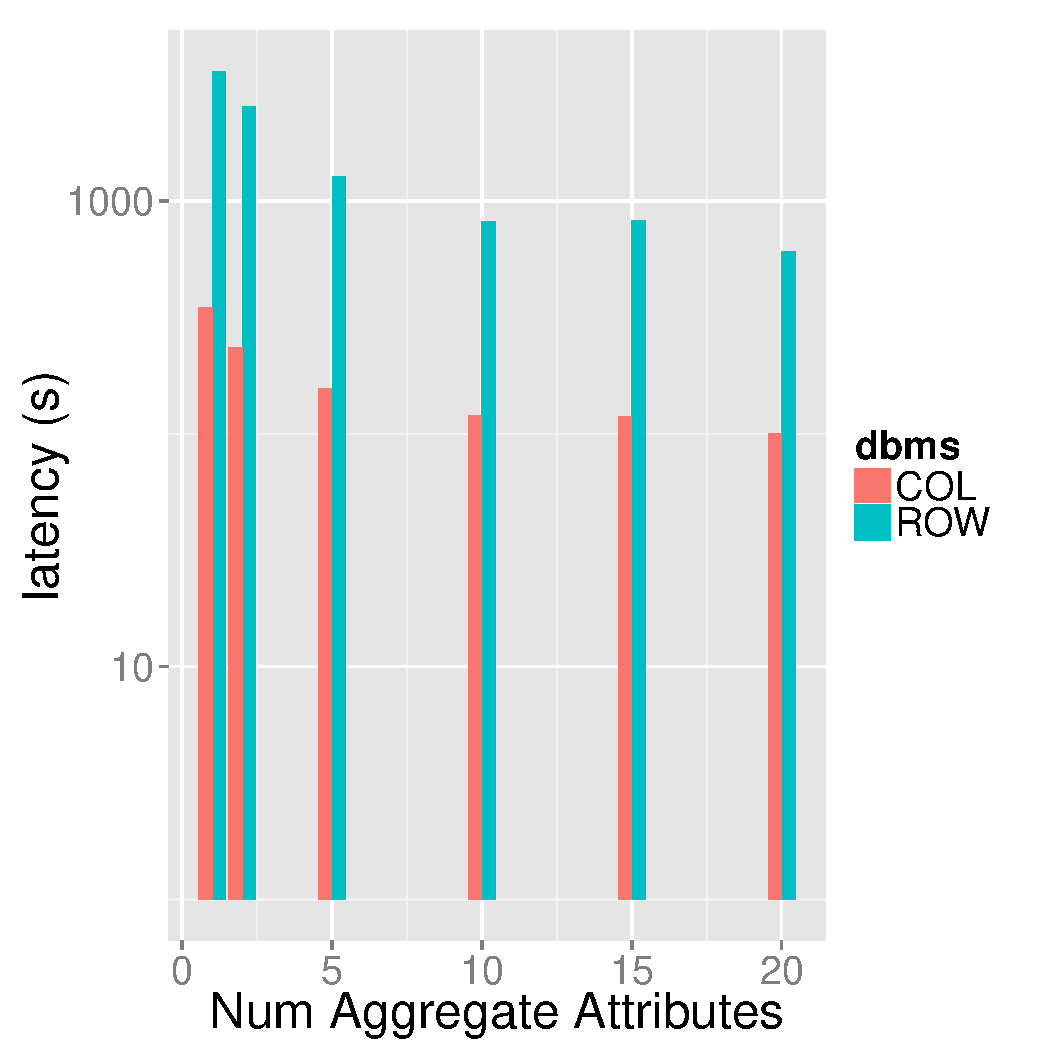
\includegraphics[width=6cm] {Images/multi_agg.pdf}}
		\caption{Latency vs. number of aggregates}
		\label{fig:multi_agg}
	\end{subfigure}
	\caption{Baseline performance and Effect of Parallel Query Execution }
	\label{fig:bank_perf}
\end{figure*}

\begin{figure*}[t]
	\centering
	\begin{subfigure}{0.33\linewidth}
		\centering
		{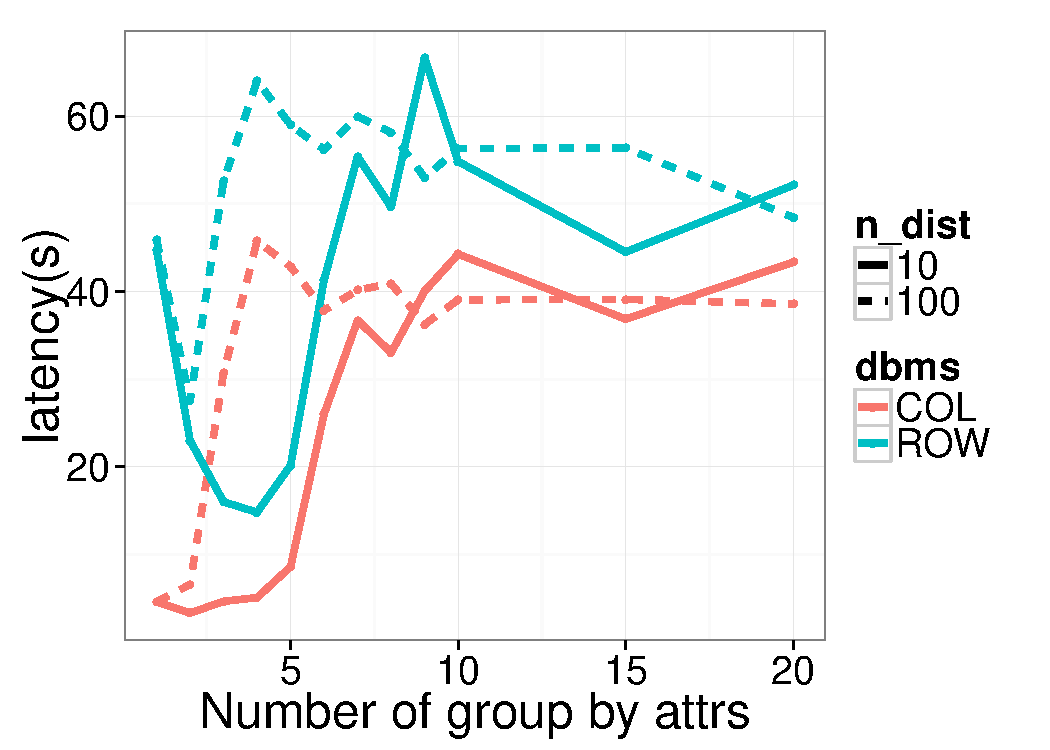
\includegraphics[width=6cm] {Images/multi_gb_same.pdf}}
		\caption{Latency vs. Num of Groups}
		\label{fig:multi_gb_same}
	\end{subfigure}
	\begin{subfigure}{0.33\linewidth}
		\centering
		{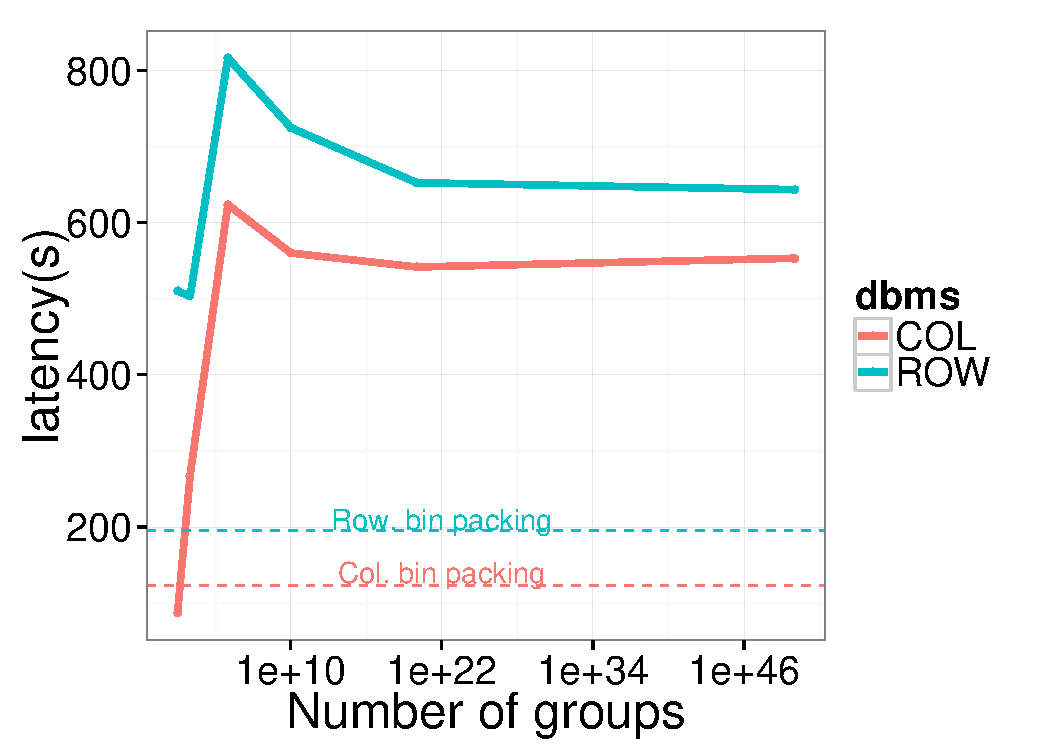
\includegraphics[width=6cm] {Images/multi_gb.pdf}}
		\caption{Latency vs. Num Dimensions}
		\label{fig:multi_gb_bp}
	\end{subfigure}
	\begin{subfigure}{0.33\linewidth}
		\centering
		{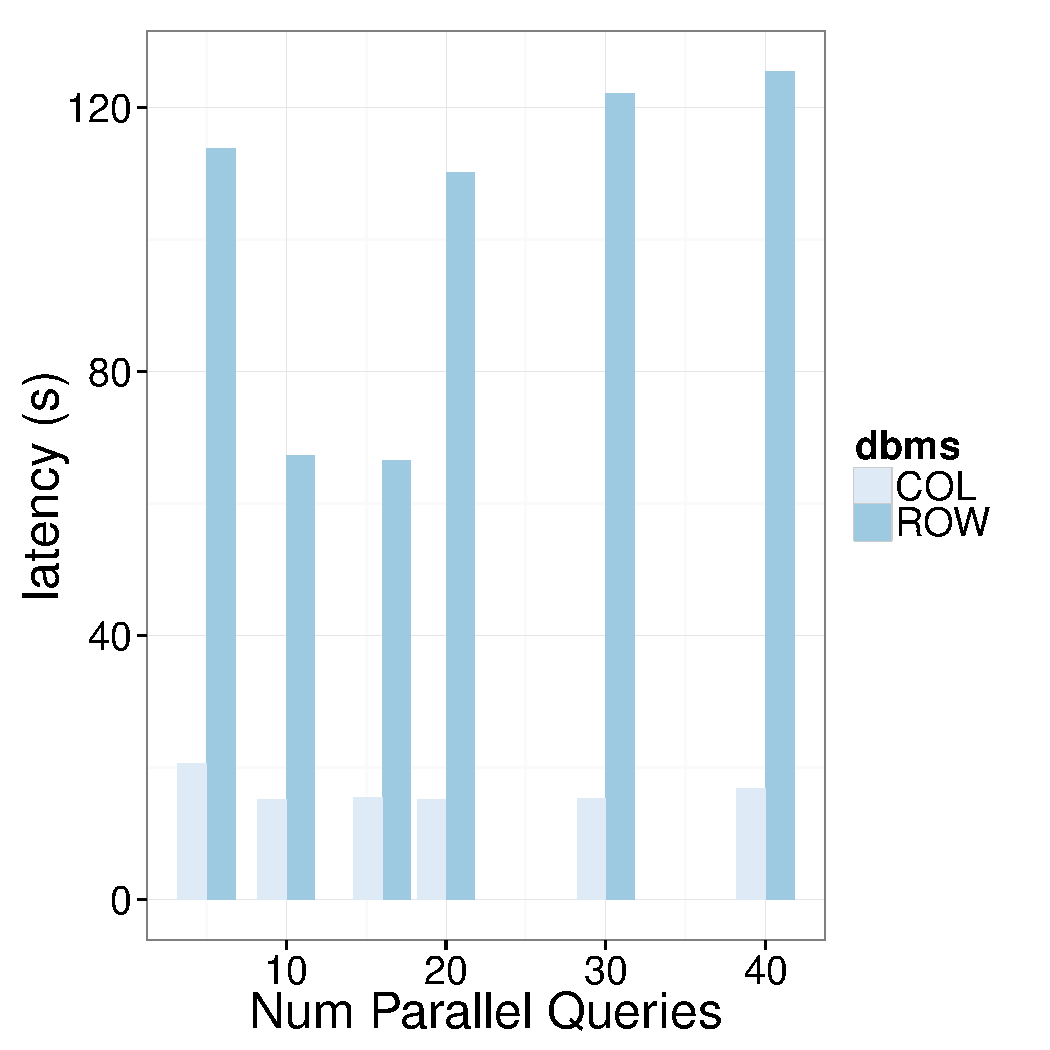
\includegraphics[width=6cm] {Images/parallel_noop.pdf}}
		\caption{Effect of parallelism}
		\label{fig:parallelism}
	\end{subfigure}
	\caption{Effect of Combining Multiple Queries \srm{Need to add a legend or mark on the figure indicating that the dotted lines are the bin packing heuristic.  Also number of groups shouldn't be out of 1e20...}}
	\label{fig:bank_perf}
\end{figure*}

\begin{figure*}[t]
	\centering
	\begin{subfigure}{0.24\linewidth}
		\centering
		{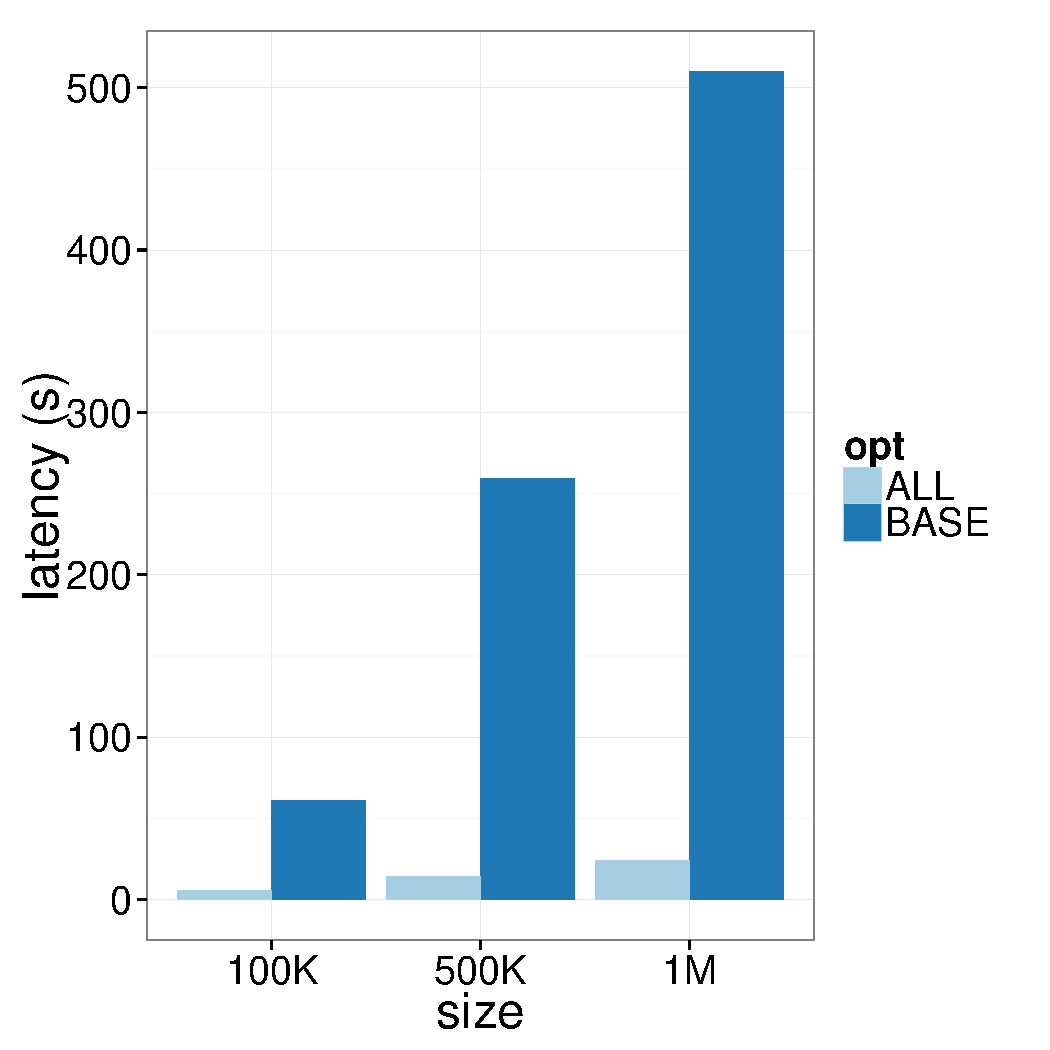
\includegraphics[width=4.6cm] {Images/row_all_none_by_size.pdf}}
		\caption{Row store latencies by vize}
		\label{fig:row_all_none_size}
	\end{subfigure}
	\begin{subfigure}{0.24\linewidth}
		\centering
		{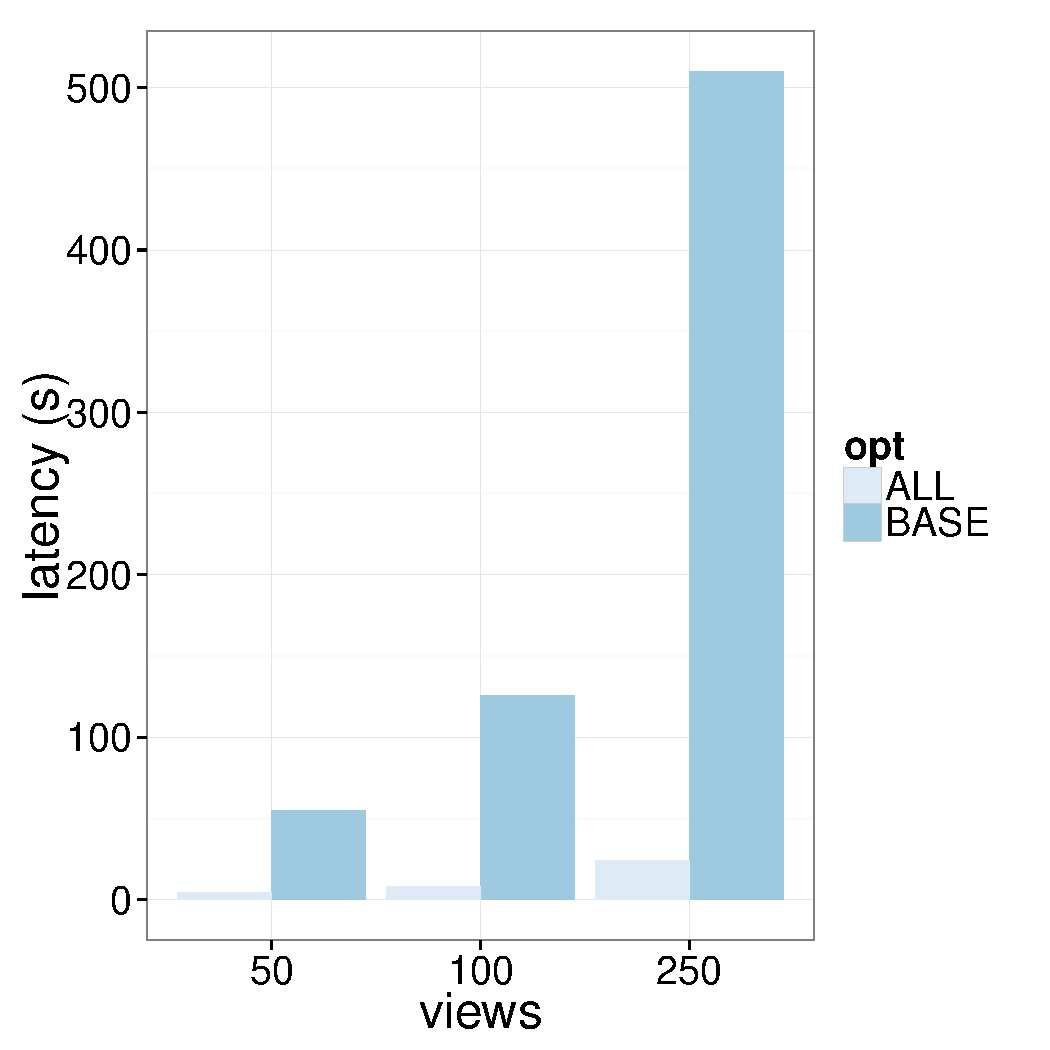
\includegraphics[width=4.6cm] {Images/row_all_none_by_views.pdf}}
		\caption{Row store latencies by views}
		\label{fig:row_all_none_views}
	\end{subfigure}
	\begin{subfigure}{0.24\linewidth}
		\centering
		{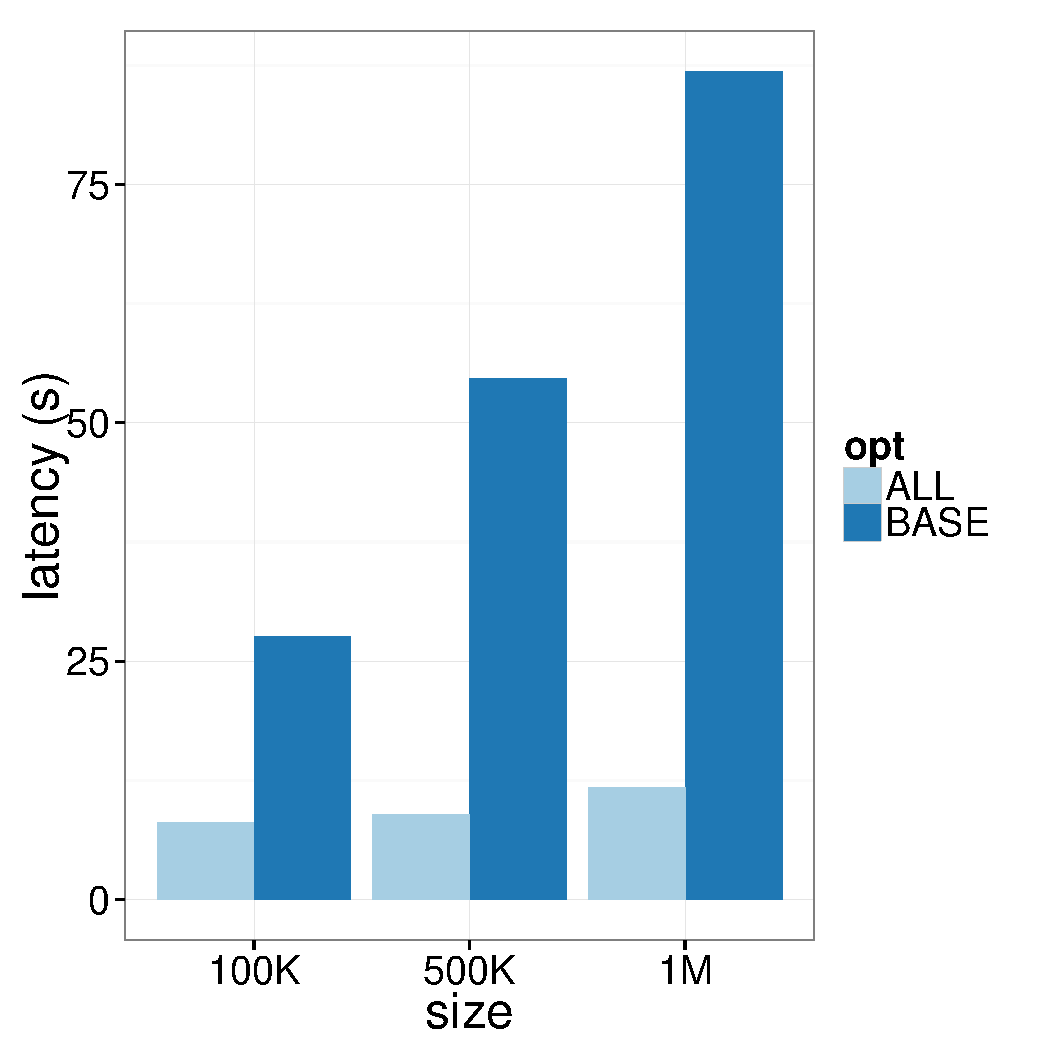
\includegraphics[width=4.6cm] {Images/col_all_none_by_size.pdf}}
		\caption{Column store latencies by size}
		\label{fig:col_all_none_size}
	\end{subfigure}
	\begin{subfigure}{0.24\linewidth}
		\centering
		{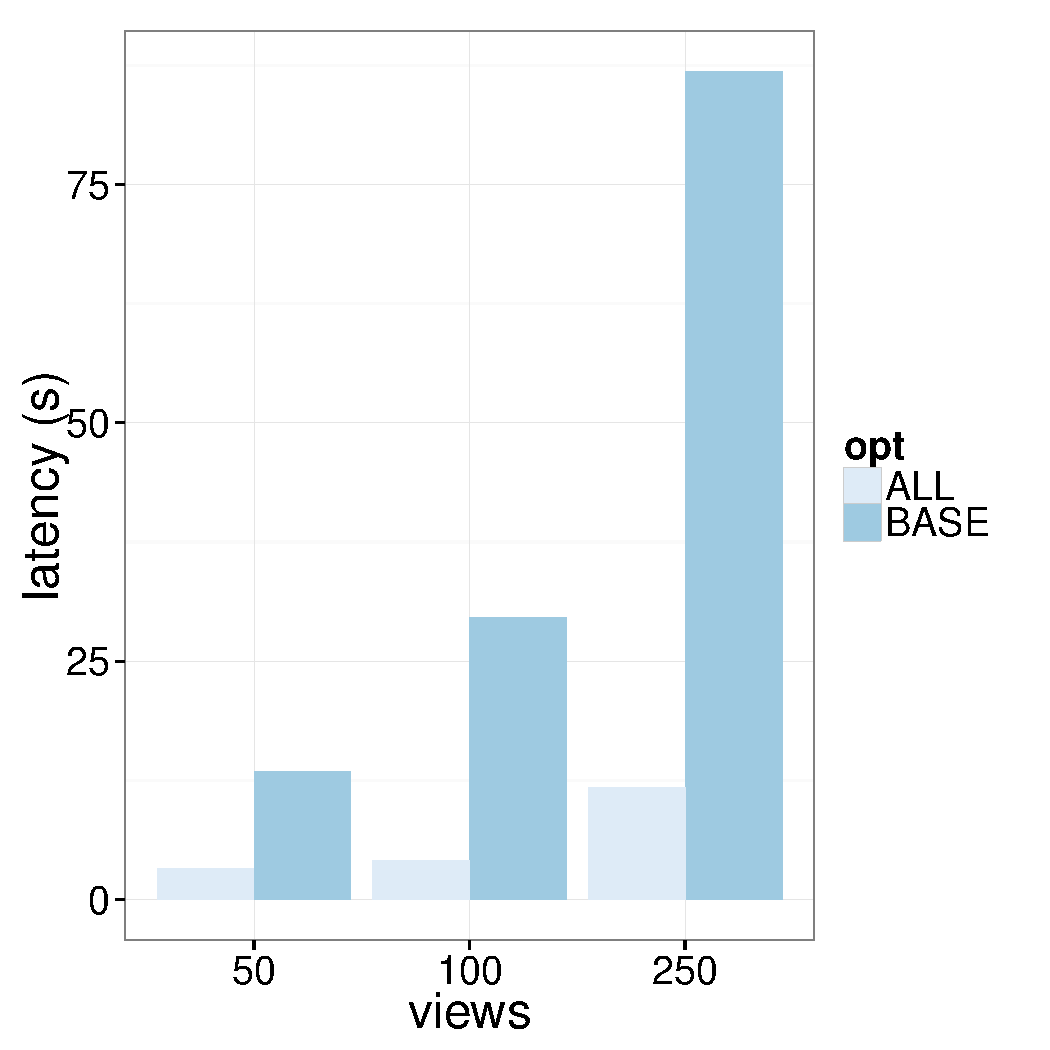
\includegraphics[width=4.6cm] {Images/col_all_none_by_views.pdf}}
		\caption{Column store latencies by views}
		\label{fig:col_all_none_views}
	\end{subfigure}
	\caption{Effect of Combining Multiple Queries \srm{Here it would be helpful to indicate the total runtime in seconds above each bar.}}
	\label{fig:all_opt}
\end{figure*}


% \begin{figure}[h]
% \centering
% \begin{subfigure}{0.49\linewidth}
% \centering
% {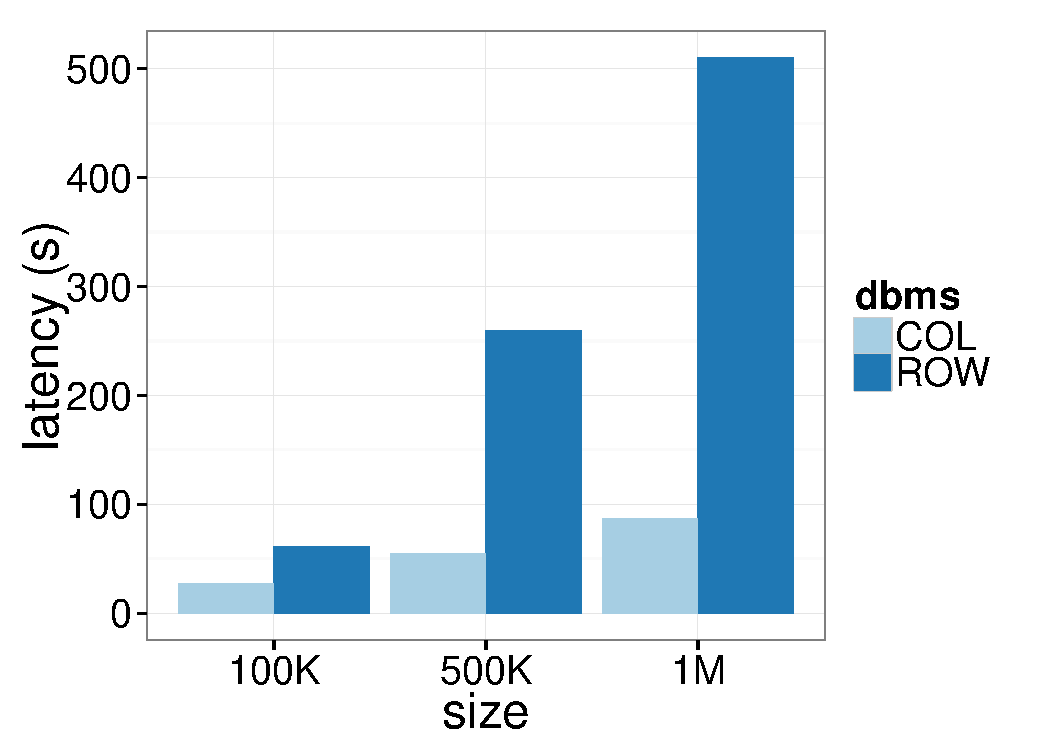
\includegraphics[width=4.2cm] {Images/baselines_by_size.pdf}}
% \caption{Latency vs. Table size}
% \label{fig:baseline_size}
% \end{subfigure}
% \begin{subfigure}{0.49\linewidth}
% \centering
% {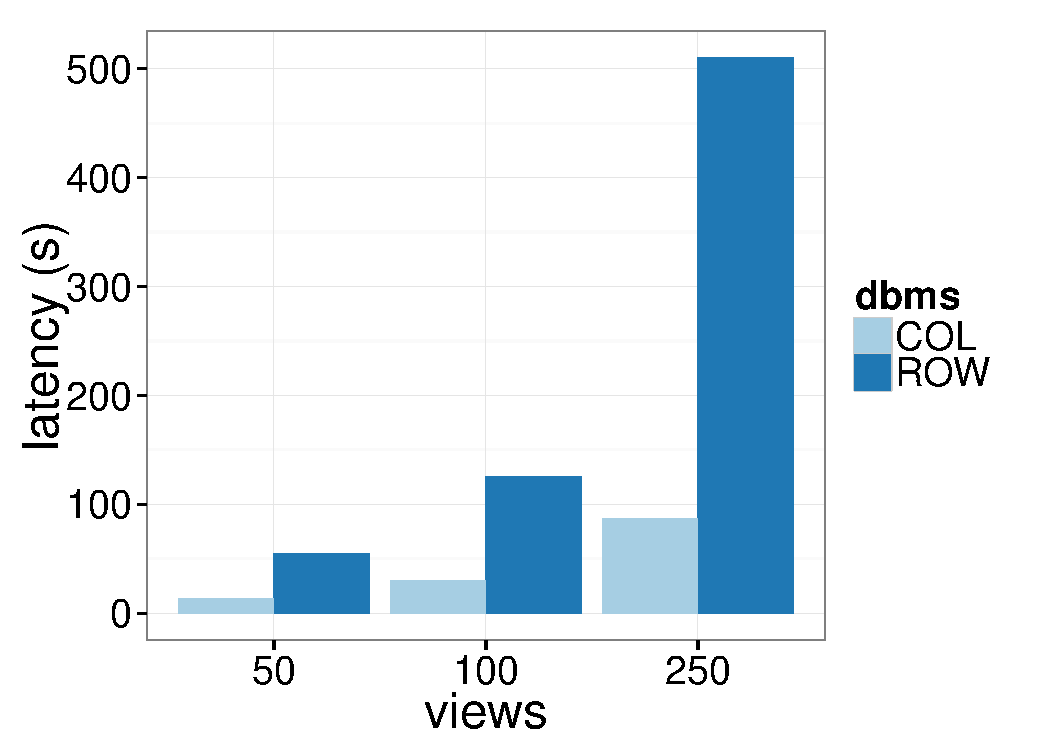
\includegraphics[width=4.2cm] {Images/baselines_by_views.pdf}}
% \caption{Latency vs. Num Views}
% \label{fig:baseline_views}
% \end{subfigure}
% \label{fig:baselines}
% \caption{Latency of Basic Framework}
% \end{figure}

\stitle{Optimization 1: Combining Multiple Aggregates:} 

{\em \underline{Summary:} Combining view queries with the same group-by attribute
but different aggregates into one query gives us a significant 
3-4X speedup for both row and column stores.}
Next, we study the impact of computing multiple aggregates within the same query,
i.e., we combine multiple view queries that have the same group-by (dimension) 
attribute, but different aggregation (measure) attributes into one query.
We ran these experiments on the SYN2 dataset 
since it has a large number (20) of measure attributes.
We varied the number of aggregate attributes ($n_{agg}$)
in a query between 1 and 20 (i.e., we grouped $n_{agg}$ view
queries that share the same group-by attribute into one query
that is issued to the DBMS).
We measured latency for each value of $n_{agg}$,
and depict the results in Figure \ref{fig:multi_agg} (log scale on the y-axis).
As we can be seen, latency drops consistently as we increase the
number of aggregations performed per query.
Notice that the latency reduction is however not quite linear in $n_{agg}$;
this may be because larger
$n_{agg}$ values require more state to the stored and, 
for column stores, more columns to be read.
Overall, this optimization shows significant speedups both in row and column stores: we
get a 4X speedup for row stores and a 3X speed up for column stores.

% \begin{figure}[h]
% \centering
% {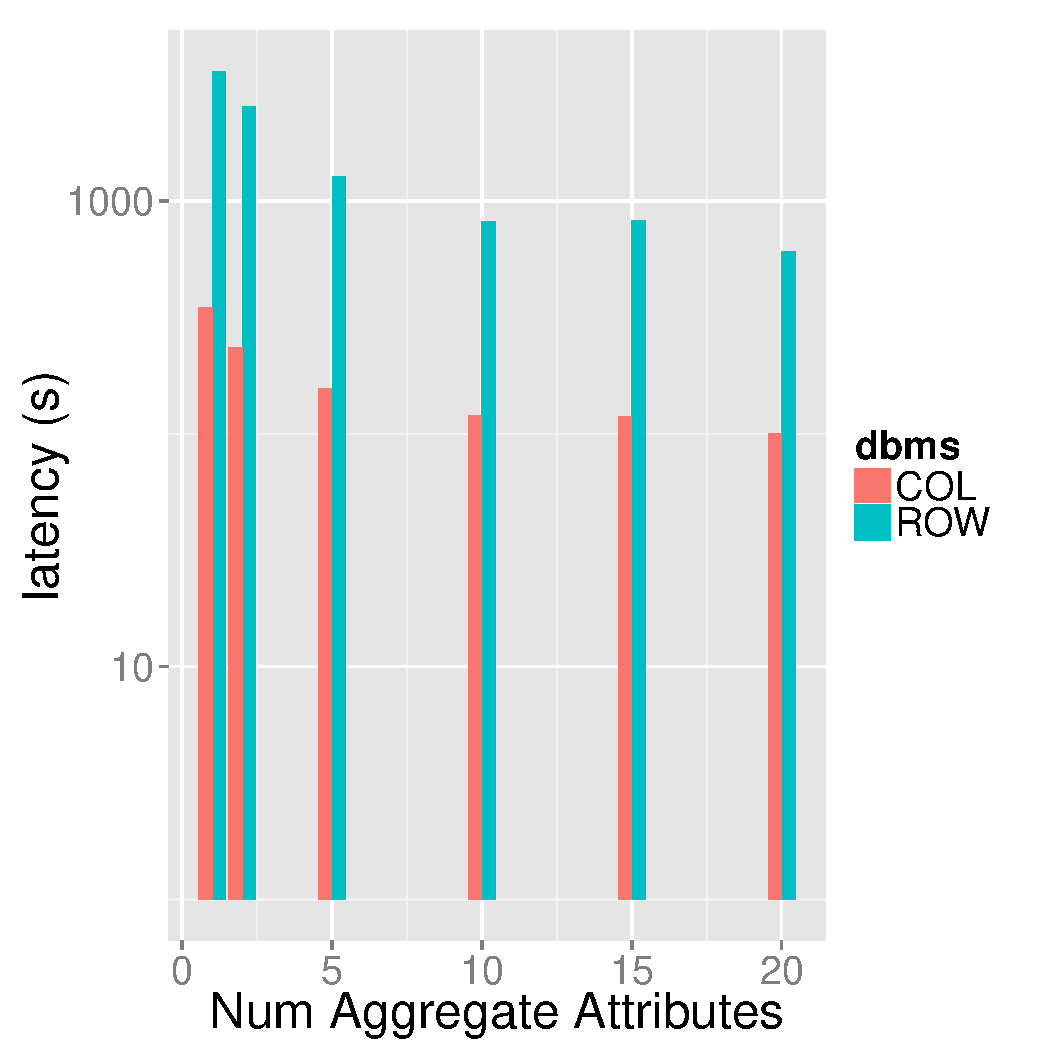
\includegraphics[width=6cm] {Images/multi_agg.pdf}}
% \caption{Latency vs. number of aggregates}
% \label{fig:multi_agg}
% \end{figure} 

\stitle{Optimization 2: Combining Multiple Group-bys:} 

{\em \underline{Summary:} Combining view queries with the same group-by attribute
but different aggregates into one query gives us a significant 
3-4X speedup for both row and column stores.}
We now study the effect of combining multiple group by attributes (with the
same dimension attribute) into one query.
In Section~\ref{sec:dbms_optimizations}, we described
how 
Section \ref{XXX} briefly discussed how the impact of this optimization was not
clear since it increases the total number of groups significantly and therefore
leads to higher costs of processing intermediate results.
To evaluate this optimization, we use the SYN3-10 and SYN3-100 datasets.
We chose these datasets over SYN1 and SYN2 since we wanted to exactly control
the number of distinct groups in every attribute and consequently the number of
distinct groups in every combination of attributes.
In SYN3-10 for example, all dimensions have 10 distinct values and each
dimension is independently generated. 
Therefore, the total number of distinct
groups produced by a query with $p$ group-by attributes is $max(10^p,
num\_rows)$.
SYN3-100 similarly has 100 distinct values per attribute and will produce
$max(10^p, num\_rows)$ groups for $p$ attributes.
Our goal in these experiments was to determine if (a) combining multiple
group-by attributes improved performance, and (b) whether it was the number of
group-by attributes or the number of distinct groups produced by a query that
predicted performance.

We ran \VizRecDB\ on SYN3-10 and SYN3-100, and varied the number of
group-by attributes in view queries ($n_{gb}$) between 1 and 20.
Figure \ref{fig:multi_gb_same} shows the results for this experiment.
We see that for the row-store, the best latency is obtained for number of
groups=$10^4$.
Beyond $10^5$, the performance degrades drastically.   \srm{same comment as
above -- we can't really have $10^{20}$ groups!} For the column-store, we see a
relatively small improvement in latency for $10^2$ groups, however, once again,
after $10^5$ groups, the performance becomes much worse.
The reason for this is as follows: as we combine group by attributes, the number
of distinct groups increases exponentially ($10^{n_{gb}}$).
As a result, the memory required for the grouping (hash-based or sort based)
also increases significantly.
Once this memory requirement exceeds the buffer space the system allocates for
intermediate results, the performance degrades significantly as the DBMS
switches to an external sort or hash algorithm.

% \begin{figure}[h]
% \centering
% \begin{subfigure}{0.49\linewidth}
% \centering
% {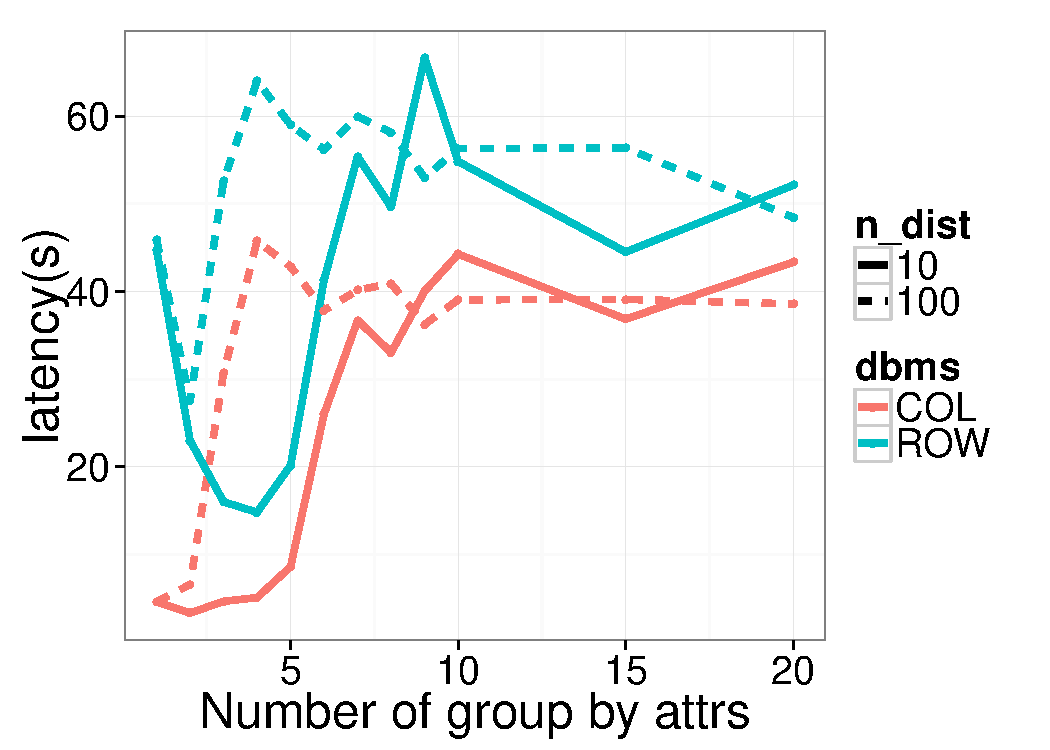
\includegraphics[width=4.2cm] {Images/multi_gb_same.pdf}}
% \caption{Latency vs. Num of Groups}
% \label{fig:multi_gb_same}
% \end{subfigure}
% \begin{subfigure}{0.49\linewidth}
% \centering
% {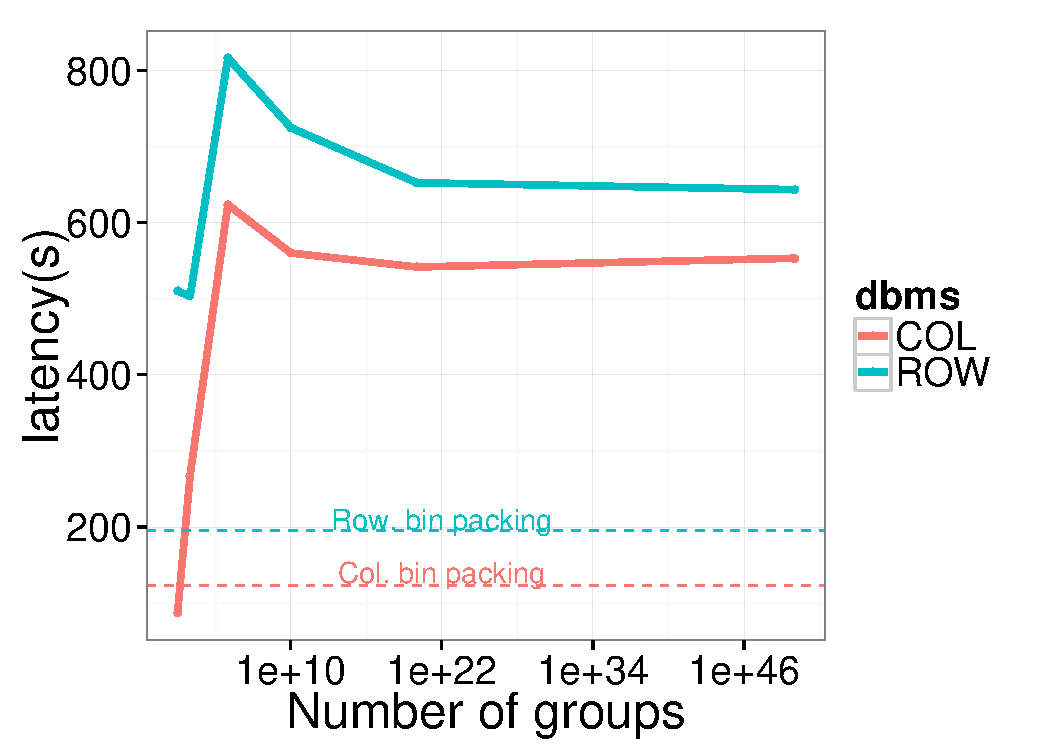
\includegraphics[width=4.2cm] {Images/multi_gb.pdf}}
% \caption{Latency vs. Num Dimensions}
% \label{fig:multi_gb_bp}
% \end{subfigure}
% \label{fig:multi_gb}
% \caption{Effect of combining multiple groups}
% \end{figure}

We can guard against the above performance degradation by ensuring that the
number of distinct groups never goes beyond a pre-configured upper limit.
From Figure \ref{fig:multi_gb_same}, we see that this limit is approximately
$10^5$ for both the row and column store.
With knowledge of this upper limit on the number of distinct groups, we can now
apply our grouping technique based on bin packing (Section \ref{}) to optimally
group the dimension attributes.
Bin-packing ensures that the number of distinct groups produced by any query is
less than $10^5$.
Figure \ref{fig:multi_gb_bp} shows the results of two grouping strategies: (a)
the bin packing-based strategy, and (b) grouping based on number of attributes.
In the latter strategy, we randomly group attributes into groups of size
$n_{gb}$. 
Since the latency for this strategy will depend on the particular grouping of
attributes, we repeated this experiment 20 times and report the average latency.
Figure \ref{fig:multi_gb_bp} shows the result for SYN1 where $n_{gb}$ was varied
between 1 and 20.
The dotted lines indicate the latency of the bin packing-based grouping strategy
whereas the solid lines indicate the latency of grouping based on attribute
number.
As we can see from the chart, bin-packing is always superior to grouping
based on attribute number.
We see that for the row-store, bin-packing reduces latency by a factor of 2X. 
What about column store???\\

\noindent {\it Parallel Query Execution}: 
Executing view queries in parallel can provide significant performance gains;
however, a high degree of parallelism can lead to a performance drop off for
several reasons. Potential reasons include disk contention, RAM usage, lock
contention, context switches and cache line contention \cite{Postgres_wiki}. 
Figure \ref{fig:parallelism} illustrates this issue: we varied the number of
queries running in parallel on the DBMS and measured the latency of
\VizRecDB.
As expected, low levels of parallelism produce sizable performance gains but
high levels of parallelism lead to degraded performance.
For our system, the optimal number of queries to run in parallel is
approximately $16$ (equal to the number of cores). 
In general, choosing a degree of parallelism equal to the number of cores
for these kinds of simple aggregation queries when data largely fits in memory
is a reasonable rule of thumb.  \\
%For other systems, we recommend users that they set the number of parallel
%queries to the maximum number of parallel queries that can be run in
%their DBMS without performance degradation.
%If this number is not easily available, a simple experiment as shown in Figure
%\ref{fig:parallelism} can help approximate the right amount of parallelism. \\

% \noindent {\it Combining Target and Comparison Views}:
% The last optimization we evaluate is that of combining the target and comparison
% views and running a single SQL query per view as opposed to two.
% We expected this optimization to roughly halve the latency since each query
% takes one table scan instead of two.\\

\noindent {\it All optimizations}:
Now that we have explored all our optimizations in detail, we pick the optimal
parameters discovered above and combine our optimizations to get the maximum
performance gain.
For the row store, we applied all the above optimizations with $n_{agg}$ set to
the number of measure attributes, maximum number of group-bys set to $10^5$ and
number of parallel queries set to $16$.
For the column store, we set $n_{agg}$ and number of parallel queries similarly
but did not apply the group-by optimization. 
Figures \ref{fig:all_opt}a-d show the latency of \VizRecDB\ on SYN1 when all
optimizations have been applied.
From Figures \ref{fig:row_all_none_size} and \ref{fig:row_all_none_views}, we
see that for the row store, our optimizations lead to a speedup of up to 20X
across a range of sizes and views.
Similarly, in Figures \ref{fig:col_all_none_size}
and \ref{fig:col_all_none_views}, we see that our optimizations lead to a 8x
speedup in columnstores. 
We also notice that our optimizations are most effective for datasets with large
sizes and many views, with proportionally larger speedups as these numbers grow.
This experiment shows that the application of well designed optimizations
can reduce \VizRecDB\ latency by 8-20X depending on the DBMS and enable a
\VizRecDB-style workload to run in interactive time scales.

In the next section, we evaluate our custom execution engine and
its pruning heuristics to evaluate the performance and accuracy implications of
pruning.

\subsection{Custom Execution Engine}
\label{sec:custom_execution_engine}

As discussed in Section \ref{}, we built a custom execution engine for
\VizRecDB\ that can share table scans across all views and use intermediate
results to prune low-utility views.  
Through the next set of experiments, we evaluate the various pruning heuristics
we developed for the custom execution engine.
Our goal is to determine the effectiveness of our strategies pruning
low-utility views and their impact on \VizRecDB\ latency.
In each of our experiments, we evaluate heuristics along three metrics:
{\it latency, accuracy} and {\it utility distance}.
As in the previous section, latency is defined as the total time taken by
\VizRecDB\ to return the top-$k$ views and is averaged over 3 runs.
Accuracy is the number of true top-$k$ views that are present in the
top-$k$ views returned by our algorithm.
Finally, utility distance is the difference between the average utility of
the true top-$k$ views and the average utility of the top-$k$ views generated by
our algorithm.
Since the accuracy and utility distance of our techniques are influenced by the
order in which data is read in, we repeat each experiment 20
times and randomize the data between runs. We report average
metrics over 20 runs.

We note that our goal is not to directly compare the latency of our custom
execution engine to the latency of the DBMS-backed execution
engine, since comparisons of completely different code bases with different
optimizations and features are nearly meaningless.  For example,
 the DBMS-backed engines (especially the column store) benefits a number of optimizations
for scan-intensive workloads, including vectorization, compression, the ability to
exploit multiple cores etc.  
Insetad, our goal is to evaluate the performance improvements that can be
obtained by pruning and sharing table scans in their own right.

% that have gone into We believe that comparing such
% systems offers little value:
% on one hand, our custom implementation lacks features such as logging or
% concurrency control that can slow down more complete systems; on the other hand,
% it also lacks optimizations for exploiting multiple cores, compression,
% vectorization, and other optimizations that scan-optimized column-stores employ.
% Rather, our goal is to highlight the relative performance benefits that can be
% obtained by performing pruning and shared scans.

Since it is hard to capture the complexities of real data distributions in synthetic data, we
evaluate all our pruning strategies on real-world data. 
Specifically, we make use of the BANK AND DIAB datasets listed in Table
\ref{tab:datasets}.
\begin{compactitem}
\item {\it Diabetes data}\cite{}: This dataset contains records of hospital
visits by patients with diabetes. Records include patient demographics,
diagnoses, number of days at the hospital, procedures performed etc. 
This dataset contains 100K records and ~80 views.
\item {\it Bank dataset}\cite{}: This dataset contains records of customers who
applied for a loan. It includes demographic information about the
customers, information about the bank's previous contact with the customer, and
the ultimate decision on the loan.
This dataset contains 40K records and ~70 views.
\end{compactitem}
We chose these datasets since they contained a mix of numerical and categorical
attributes and were comparable to other analytical datasets in size.

For each of the above datasets, we evaluate 4 pruning strategies:
\begin{compactenum}[(a)]
\item No Pruning (NO\_PRU): we make a single pass of the data and keep running
estimates for the utility of every possible view. Once we have seen all the
data, we return the top-$k$ views with highest utility; \item Hoeffding Intervals
(HOEFF):
we use pruning based on Hoeffding intervals (Section \ref{}); \item 95\%
Confidence Intervals (95\_CI): we use pruning based on 95\% confidence intervals
(Section \ref{}); and \item Multi-armed Bandit (MAB): we perform pruning based on
the multi-armed bandit formulation (Section \ref{}).
For each of our datasets, we varied $k$, the number of views to select, between
1 and 25 (a realistic upper limit on the number of views displayed to the user)
and measured the latency, accuracy and utility distance for each of our
heuristics.
\end{compactenum}

We begin with an evaluation of our techniques with respect to their accuracy
and utility distance.\\

\begin{figure}[h]
	\centering
	\begin{subfigure}{1\linewidth}
		\centering
		{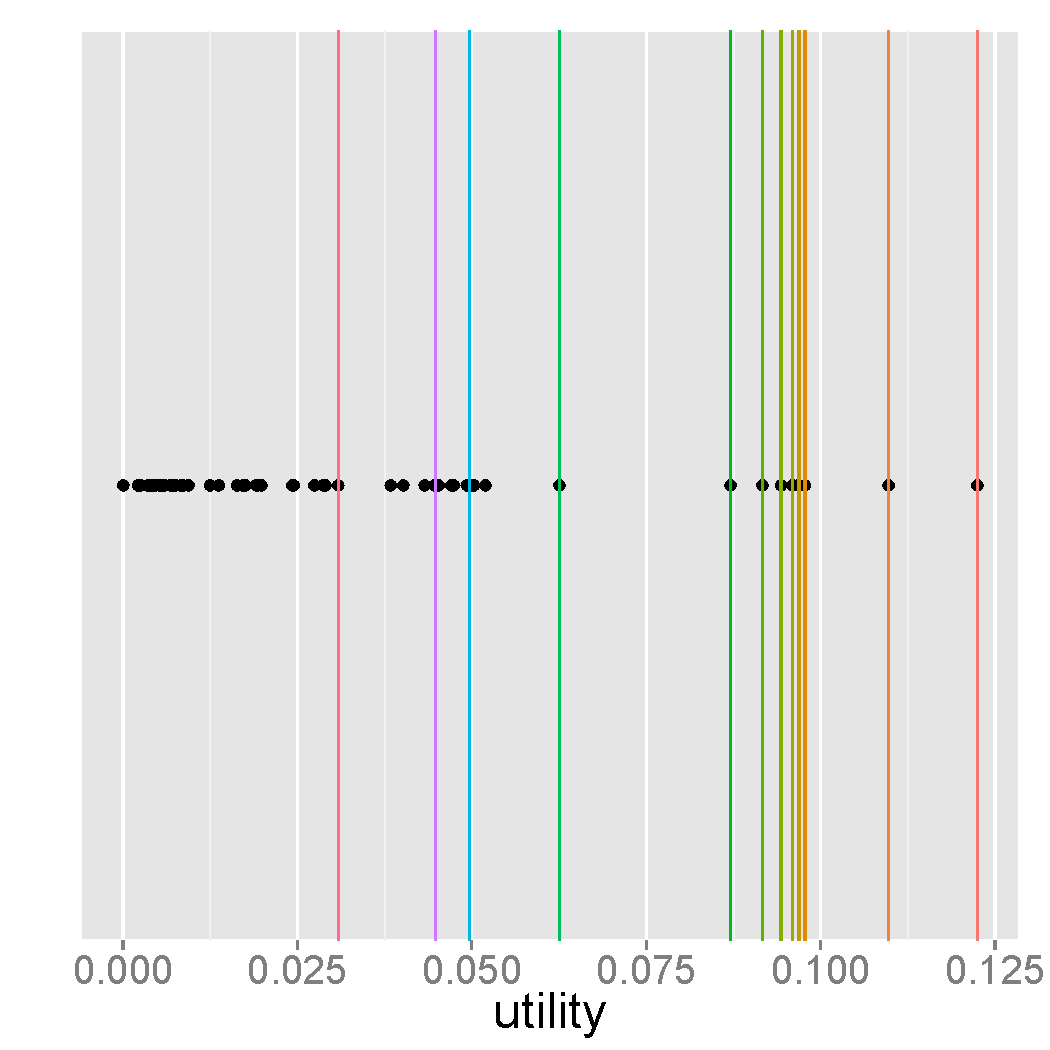
\includegraphics[trim = 0mm 60mm 0mm 60mm, clip, width=8cm]
		{Images/bank_utility_distribution.pdf}}
		\caption{Bank dataset: utility distribution}
		\label{fig:bank_utility_distribution}
	\end{subfigure}
	
	\begin{subfigure}{1\linewidth}
		\centering
		{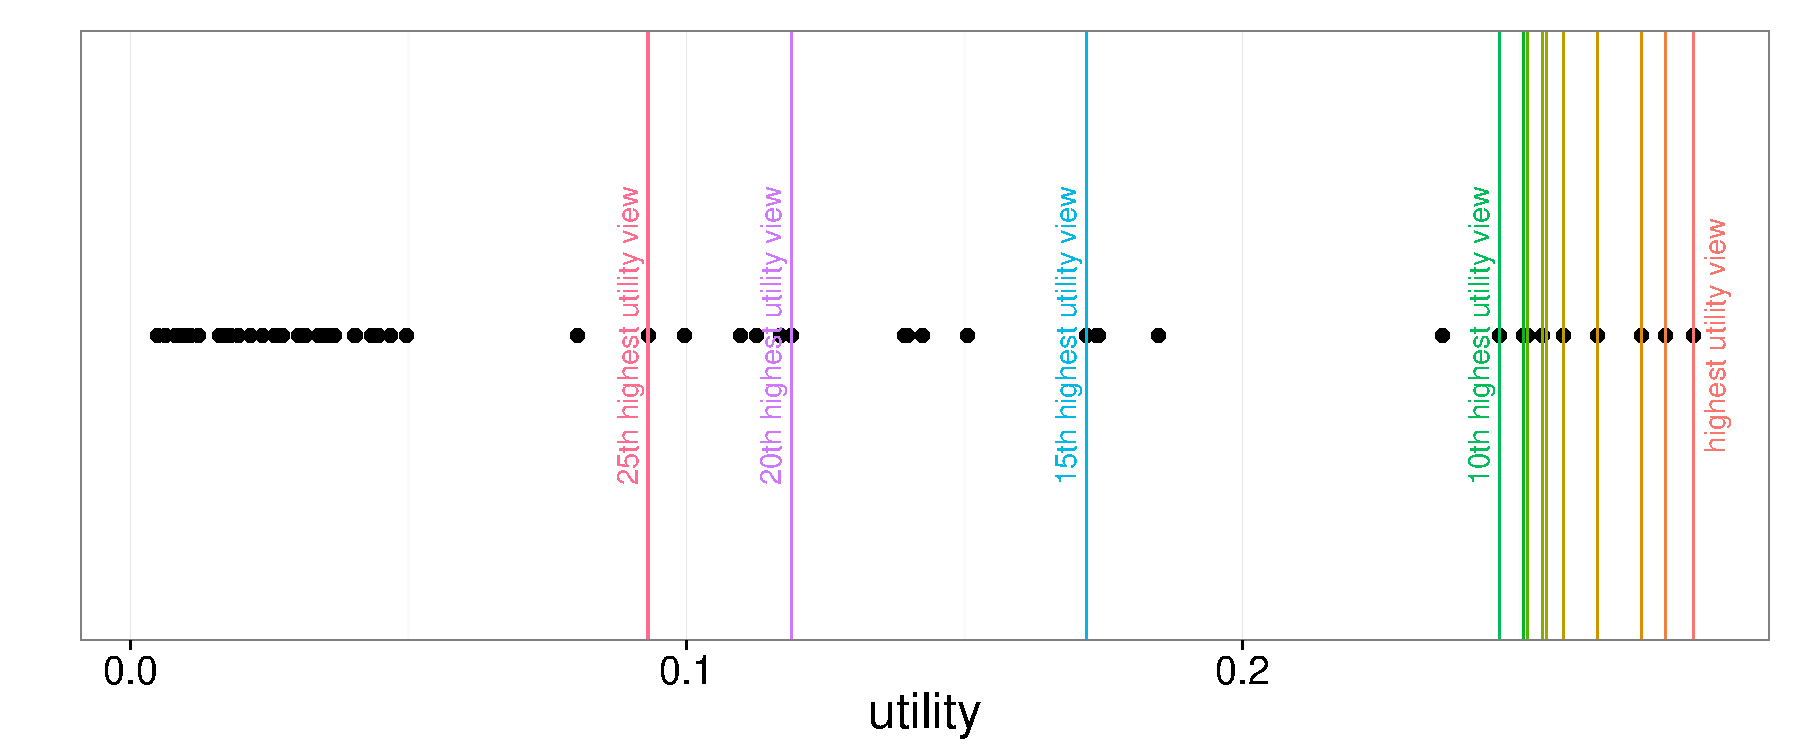
\includegraphics[trim = 0mm 60mm 0mm 60mm, clip, width=8cm]
		{Images/diabetes_utility_distribution.pdf}}
		\caption{Diabetes dataset: utility distribution}
		\label{fig:diabetes_utility_distribution}
	\end{subfigure}
\label{fig:utility_distribution}
\caption{Distribution of Utilities \srm{Need to show the absolute utility values and sequence number of the bars/dots in this figure}}
\end{figure}


\noindent {\it Accuracy and Utility Distance}:
We start with the banking dataset.
The distribution of utilities for all views of the banking dataset is
shown in Figure \ref{fig:bank_utility_distribution}. 
In this chart, vertical lines denote the cutoffs for utilities for top-$k$ views
where $k$=\{1\ldots10,15,20,25\}.
The highest utility for this dataset corresponds to the {\it right-most} line
in this chart while the 25-th highest utility corresponds to the {\it left-most}
line.
From the chart we see that the
highest and second highest utility are spread well apart from the rest of the
utilities.
We also observe that the top 3rd--9th utilities are rather similar. 
The 10th highest utility is again separated from neighboring utilities by a
large value and then the remaining utilities are again close together.
This distribution of utilities directly impacts the performance of our pruning
techniques since utilities that are close together have very similar running
estimates of utility and hence are difficult to tease apart and prune.
Utilities that are spread apart, in contrast, have estimates that are also
spread apart and we can prune views easily.

We see that the impact of this utility distribution in the accuracy chart in
Figure \ref{fig:bank_accuracy}.
We find that the average accuracy of all three heuristics is reasonable for
$k$=1 and 2 (recall that these are spread apart from the other utilities).
However, between $k$=3\ldots9, the accuracy suffers (consequence of similar
utility values).
After $k$=10, the performance of all our heuristics improves once again.

Now, let us examine how ``bad'' our errors are in finding the top-$k$ views.
We do so by looking at the utility distance (i.e. the distance between
the average utility of the true top-$k$ views and the average utility of the
top-$k$ views picked by our strategies).
Utility distance gives us an easy way to measure how far we are from the true
top-$k$ views.
Figure \ref{fig:bank_utility_dist} shows the utility distance for
all of our heuristics for the bank dataset.
The NO\_PRU technique necessarily has 0 utility distance since
it performs no pruning.
We add an extra ``strategy'' here which is the random strategy (RANDOM).
It essentially means that we chose any $k$ views at random and computed their
utility distance.
This strategy serves as a lowerbound on the quality of our results.
Notice that all of our heuristics are significantly better than the RANDOM
strategy for all $k$s.
All of our heuristics produce views with 0 or almost 0 utility distance. 
Thus, there is effectively no difference in the utilities of the top $k$ views
we select vs. the true top-$k$ views.
So even when a top-$k$ strategy picks a few incorrect views, the selected views
have utility very close to the real top-$k$ views, i.e., are views are
approximate but of high quality.
% This implies that even if our top-$k$ views are
% approximate, they are of high quality.
% Another way to analyze mistakes in the top-$k$ views is by examining if the an
% incorrectly returned view for the top-$k$ views also appears in the top-$2k$,
% top-$3k$ or top-$4k$.
% Figure \ref{} shows the results for the banking dataset.
% We see that XXX,

\begin{figure*}[t]
	\centering
	\begin{subfigure}{0.33\linewidth}
		\centering
		{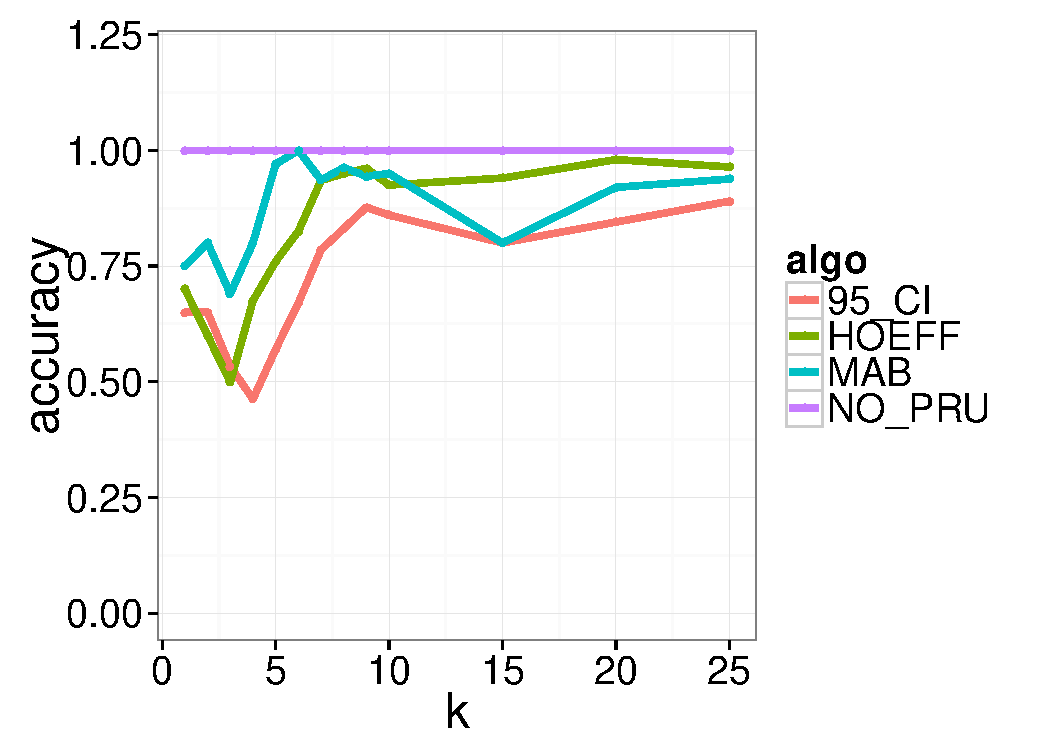
\includegraphics[width=6cm] {Images/in_memory_bank_accuracy.pdf}}
		\caption{Accuracy}
		\label{fig:bank_accuracy}
	\end{subfigure}
	\begin{subfigure}{0.33\linewidth}
		\centering
		{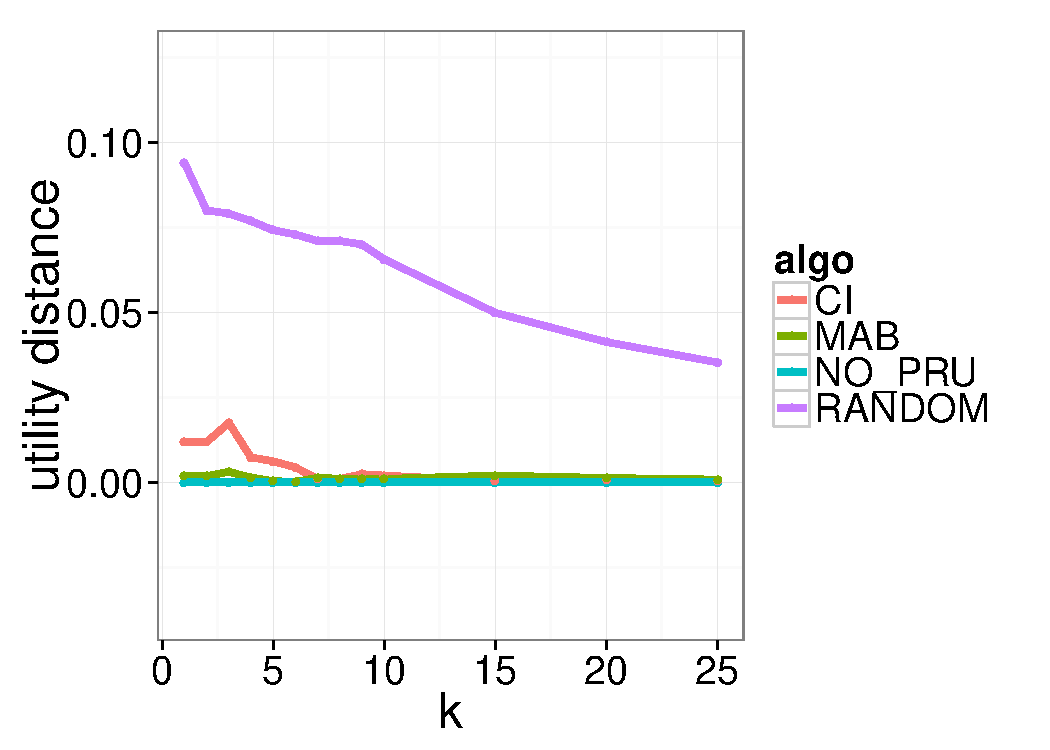
\includegraphics[width=6cm] {Images/in_memory_bank_utility_dist.pdf}}
		\caption{Utility Distance}
		\label{fig:bank_utility_dist}
	\end{subfigure}
	\begin{subfigure}{0.33\linewidth}
		\centering
		{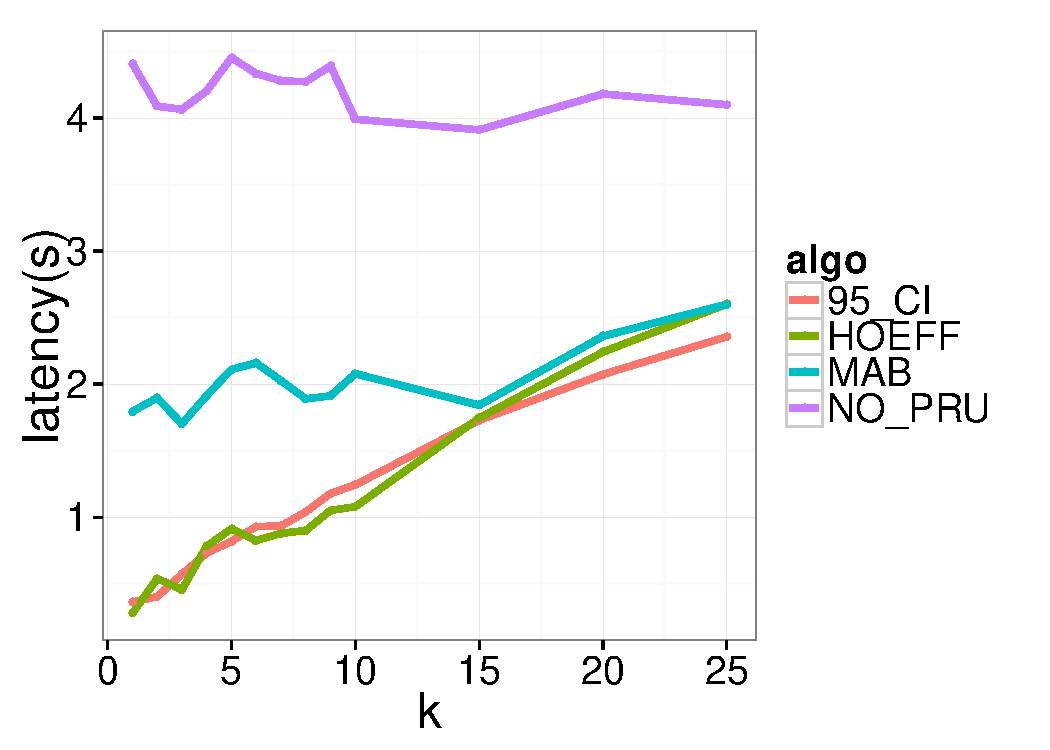
\includegraphics[width=6cm] {Images/in_memory_bank_latency.pdf}}
		\caption{Latency}
		\label{fig:bank_latency}
	\end{subfigure}
	\caption{Performance of heuristics for Bank dataset}
	\label{fig:bank_perf}
\end{figure*}

\begin{figure*}[t]
	\centering
	\begin{subfigure}{0.33\linewidth}
		\centering
		{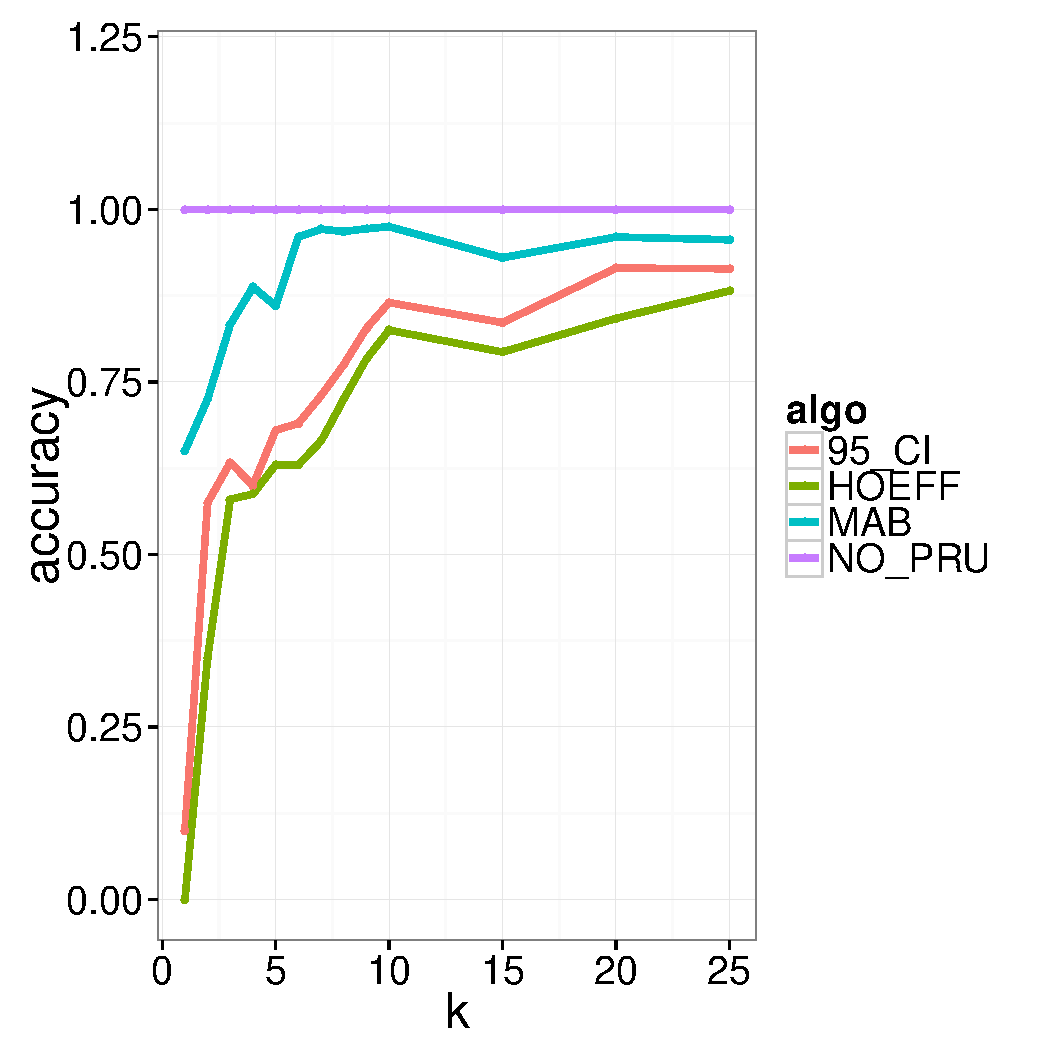
\includegraphics[width=6cm] {Images/in_memory_dia_accuracy.pdf}}
		\caption{Accuracy}
		\label{fig:dia_accuracy}
	\end{subfigure}
	\begin{subfigure}{0.33\linewidth}
		\centering
		{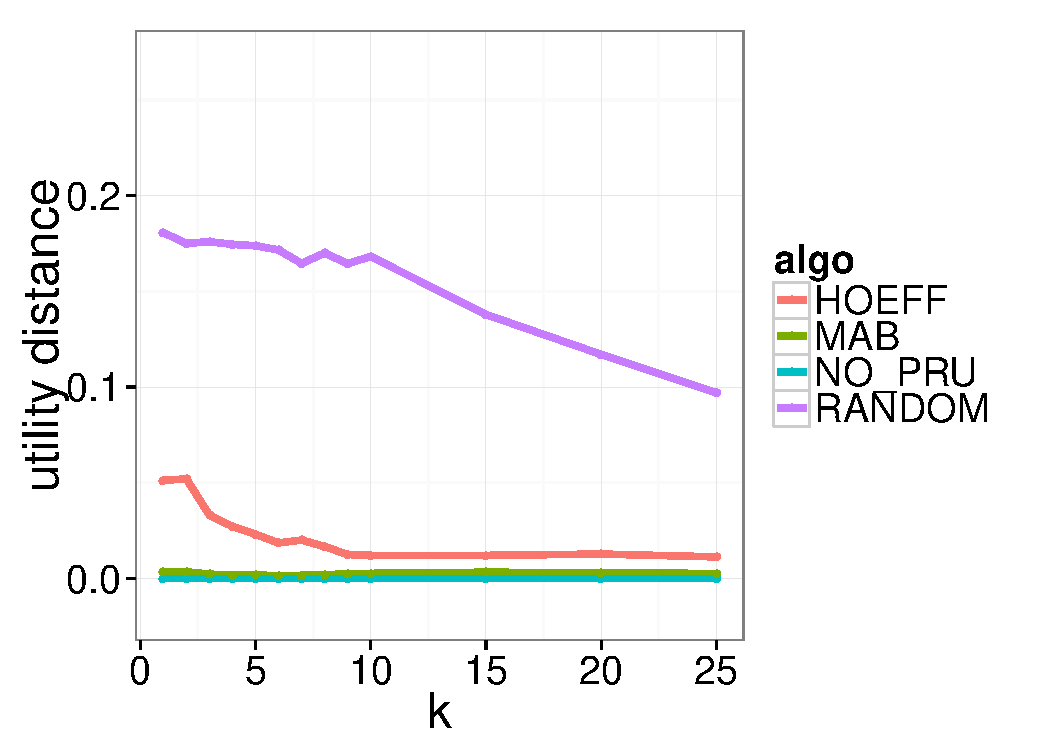
\includegraphics[width=6cm] {Images/in_memory_dia_utility_dist.pdf}}
		\caption{Utility Distance}
		\label{fig:dia_utility_dist}
	\end{subfigure}
	\begin{subfigure}{0.33\linewidth}
		\centering
		{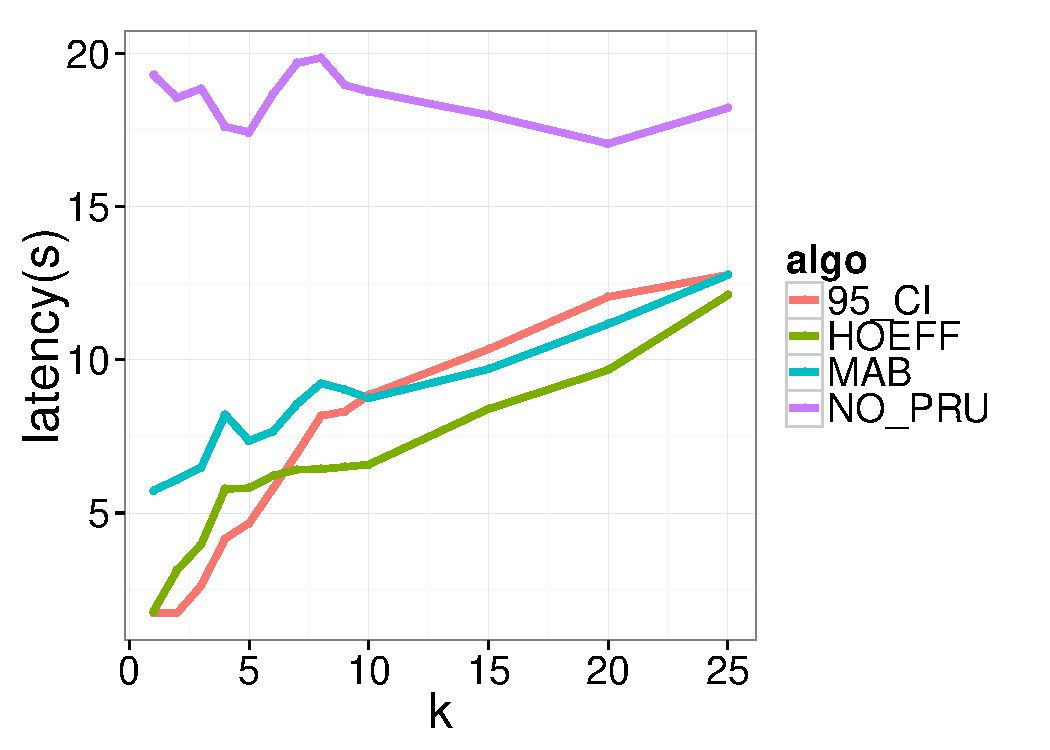
\includegraphics[width=6cm] {Images/in_memory_dia_latency.pdf}}
		\caption{Latency}
		\label{fig:diabetes_latency}
	\end{subfigure}
	\caption{Performance of heuristics for Diabetes dataset}
	\label{fig:diabetes_perf}
\end{figure*}

% \begin{figure}[h]
% \centering
% \begin{subfigure}{0.49\linewidth}
% \centering
% {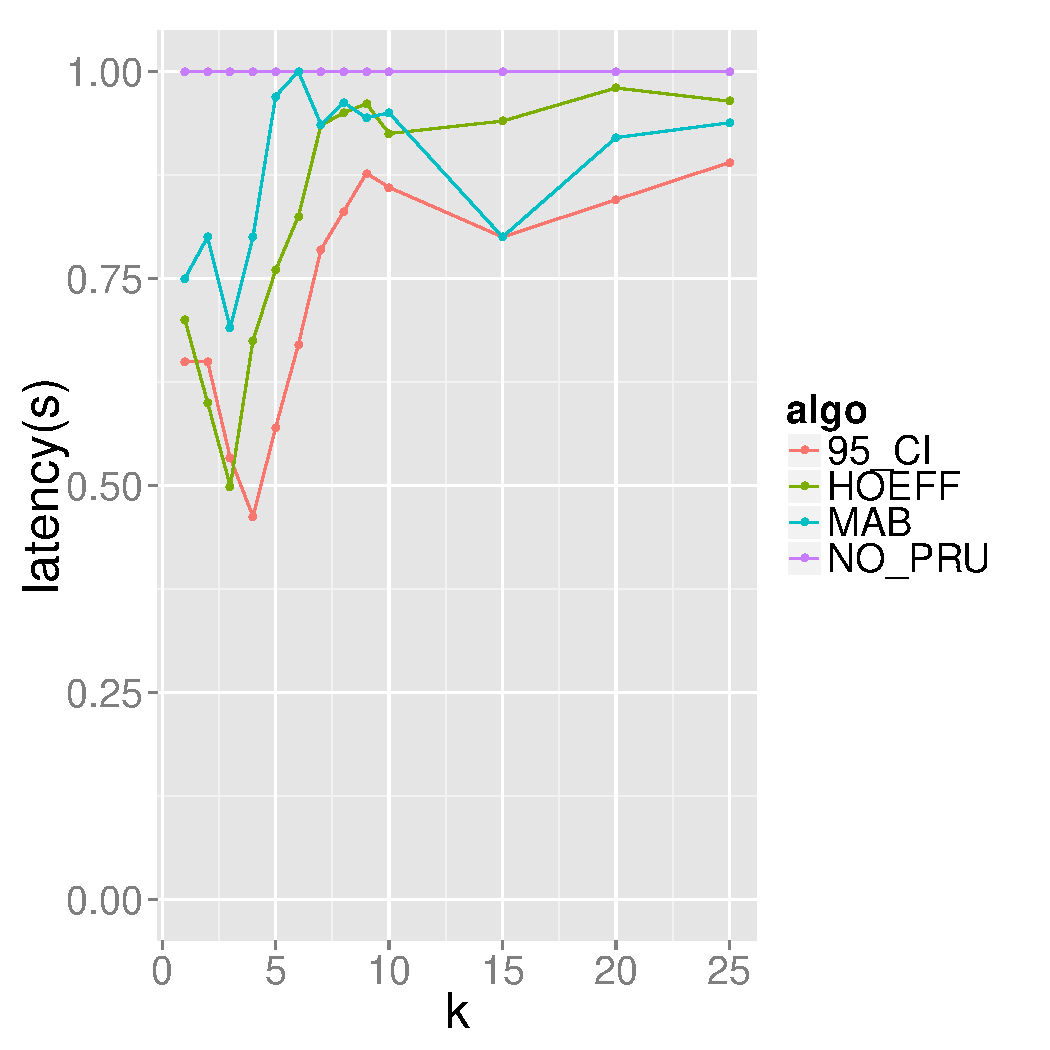
\includegraphics[width=4.2cm] {Images/bank_in_memory_accuracy.pdf}}
% \caption{Accuracy of heuristic for bank dataset}
% \label{fig:bank_accuracy}
% \end{subfigure}
% \begin{subfigure}{0.49\linewidth}
% \centering
% {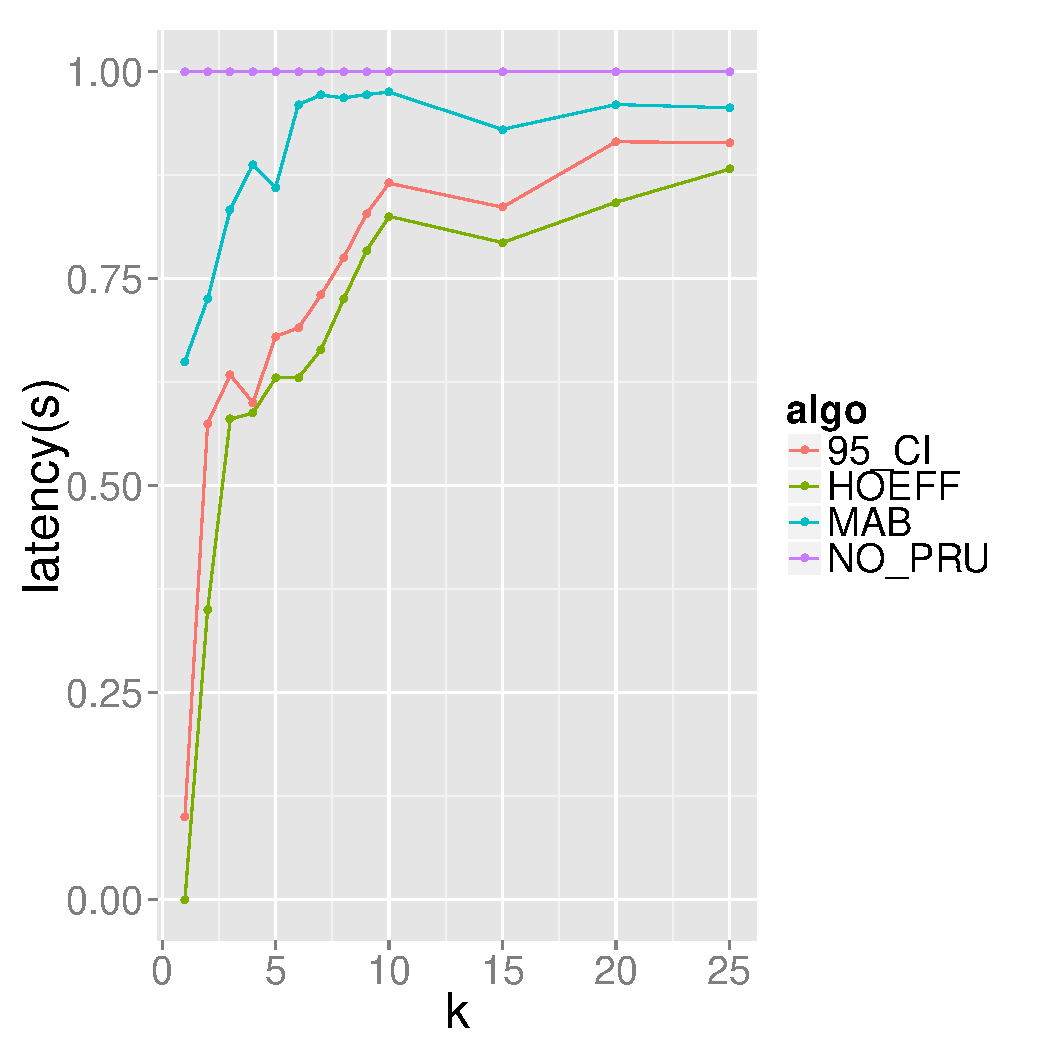
\includegraphics[width=4.2cm] {Images/dia_in_memory_accuracy.pdf}}
% \caption{Accuracy of heuristics for diabetes dataset}
% \label{fig:dia_accuracy}
% \end{subfigure}
% \label{fig:accuracy}
% \caption{Accuracy of Heuristics}
% \end{figure}


% \begin{figure}[h]
% \centering
% \begin{subfigure}{0.49\linewidth}
% \centering
% {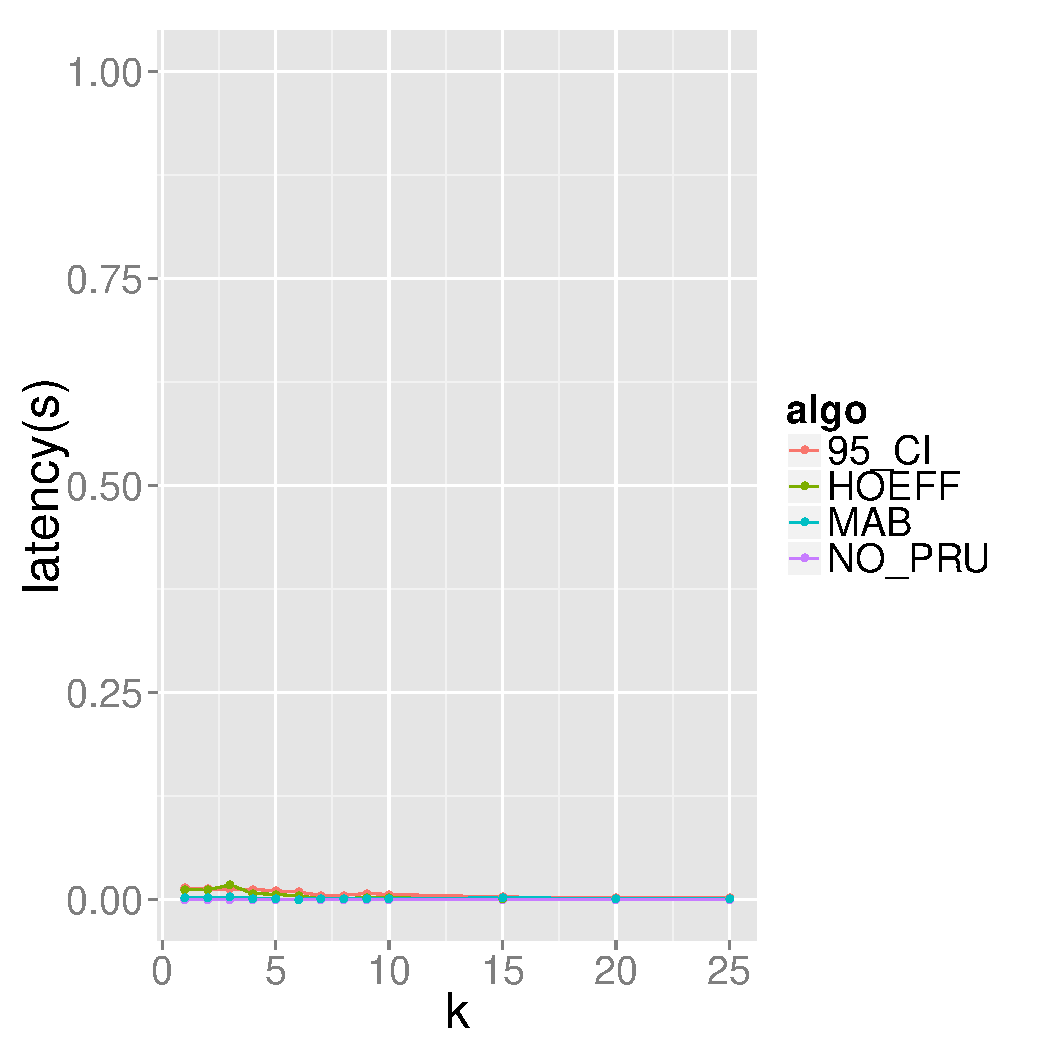
\includegraphics[width=4.2cm] {Images/bank_in_memory_utility_dist.pdf}}
% \caption{Utility Distance of heuristic for bank dataset}
% \label{fig:bank_utility_dist}
% \end{subfigure}
% \begin{subfigure}{0.49\linewidth}
% \centering
% {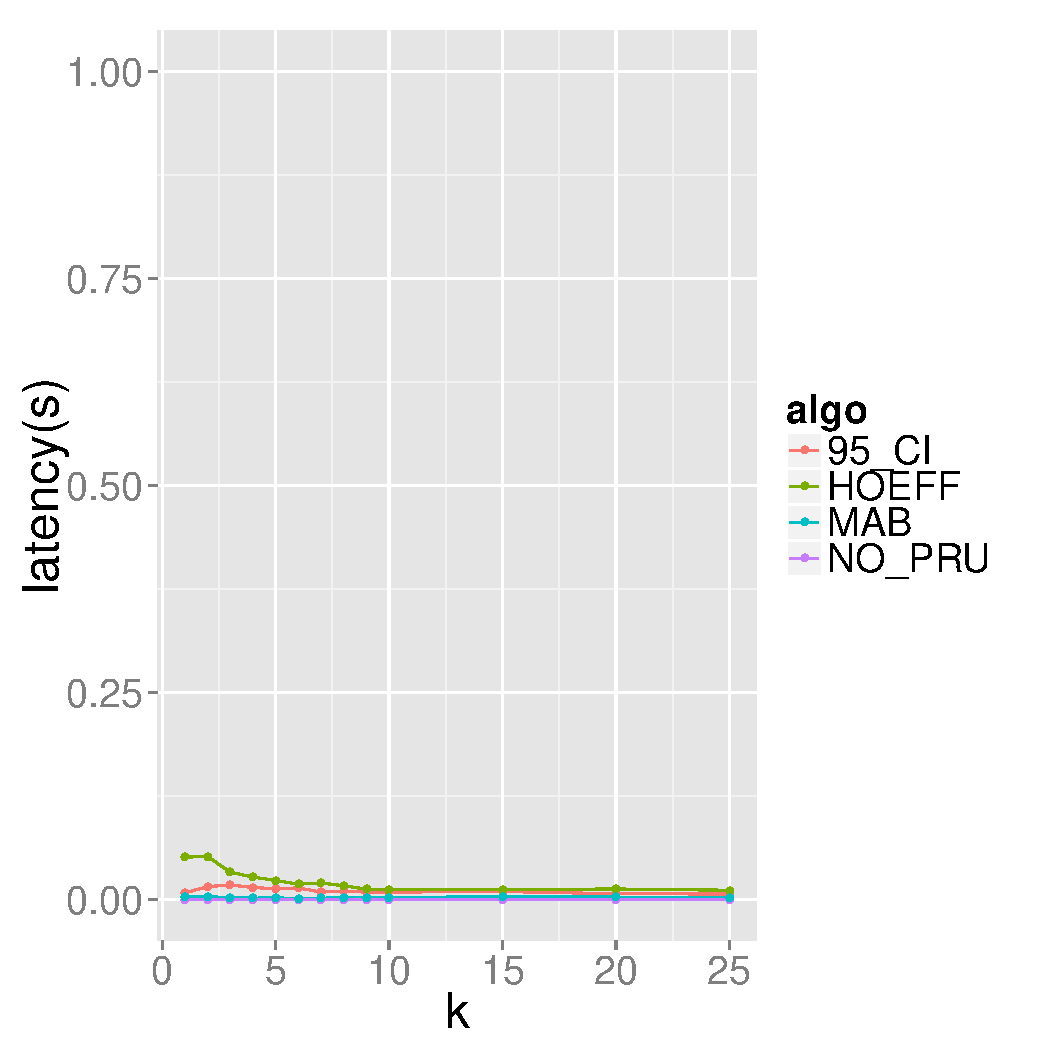
\includegraphics[width=4.2cm] {Images/dia_in_memory_utility_dist.pdf}}
% \caption{Utility Distance of heuristics for diabetes dataset}
% \label{fig:dia_utility_dist}
% \end{subfigure}
% \label{fig:accuracy}
% \caption{Utility Distance for Heuristics}
% \end{figure}

% \begin{figure}[h]
% \centering
% {\includegraphics[trim = 0mm 50mm 0mm 50mm, clip, width=6cm]
% {Images/bank_utility_distribution.pdf}}
% \caption{Bank dataset: utility distribution}
% \label{fig:bank_utility_distribution}
% \end{figure}
% \begin{figure}[h]
% \centering
% {\includegraphics[trim = 0mm 50mm 0mm 50mm, clip, width=6cm]
% {Images/diabetes_utility_distribution.pdf}}
% \caption{Diabetes dataset: utility distribution}
% \label{fig:diabetes_utility_distribution}
% \end{figure}
 
Next, let us examine the results for the diabetes dataset.
The distribution of true utilities for all views in this dataset are shown in
Figure \ref{fig:diabetes_utility_distribution}.
Compared to the bank dataset, we see that utilities are very closely
clustered for top 1\ldots10 views.
On the other hand, the utilities around $k$=15, 20 and 25 are relatively widely
spaced.
As a result, we expect lower pruning accuracy for $k<10$ but high accuracy for
large $k$'s.
We see this behavior in Figure \ref{fig:dia_accuracy} where the accuracy of
pruning is quite low for small $k$s, increases until $k$=10 and then levels off.
A similar trend is seen in Figure \ref{fig:dia_utility_dist} showing that
utility distance is small for $k<10$ and then reduces to almost 0 for larger
$k$s.

We also observe an important property of our heuristics: the accuracy of all
three of our heuristics, MAB, 95\_CI and HOEFF, is comparable; MAB appears to
perform better for small number of $k$s but all three produce similar results
for $k>10$. (NO\_PRU is guaranteed to have perfect accuracy).
This suggests that since all heuristics perform similarly on accuracy, we can
choose the heuristic with the minimum latency.\\

% 95\_CI does the best among all our heuristics for the whole range of $k$ values.
% MAB and HOEFF produce similar accuracy values with MAB being slightly better
% than HOEFF.
% There are a few reasons why 95\_CI performs better: the MAB heuristic is tied to
% either accepting or discarding a view at the end of each phase; therefore, even
% if MAB is not very confidence in the action of accepting or discarding, it must
% reduce one view in each phase. HOEFF on the other hand is less accurate because
% XXX.
% All our heuristics however seem to have low accuracy for $k<10$. 

\noindent {\it Latency}:
Next, let us look at how long it takes for each of our pruning strategies to
work.
Figures \ref{fig:bank_latency} and \ref{fig:diabetes_latency} show the latency
of our heuristics for the banking and diabetes dataset.
The two charts look quite similar.
First off, we observe that {\it the use of any of our heuristics reduces the
latency by about 50\%}.
For NO\_PRU and 95\_CI, for small $k$'s, we obtain almost a 90\% reduction in
latency. However, as we saw earlier, some of this reduction in latency is
obtained at the cost lower accuracy.
We observe that the latency of HOEFF and 95\_CI increases almost linearly
with $k$.
Roughly speaking, this trend arises because as $k$
increases, we throw out fewer views and therfore perform more
computation per record.
This exact trend is not seen in MAB because MAB's pruning of views is agnostic
to the number of views that must be selected.

In general, we see that it is possible to reduce latency by 50\% just by using
any of our heuristics.
In fact, if we are willing to tradeoff some accuracy, we can cut latency by
90\%.
The next set of experiments vary the parameters for each heuristic to study
the accuracy vs. latency tradeoff.\\

% \begin{figure}[h]
% \centering
% \begin{subfigure}{0.49\linewidth}
% \centering
% {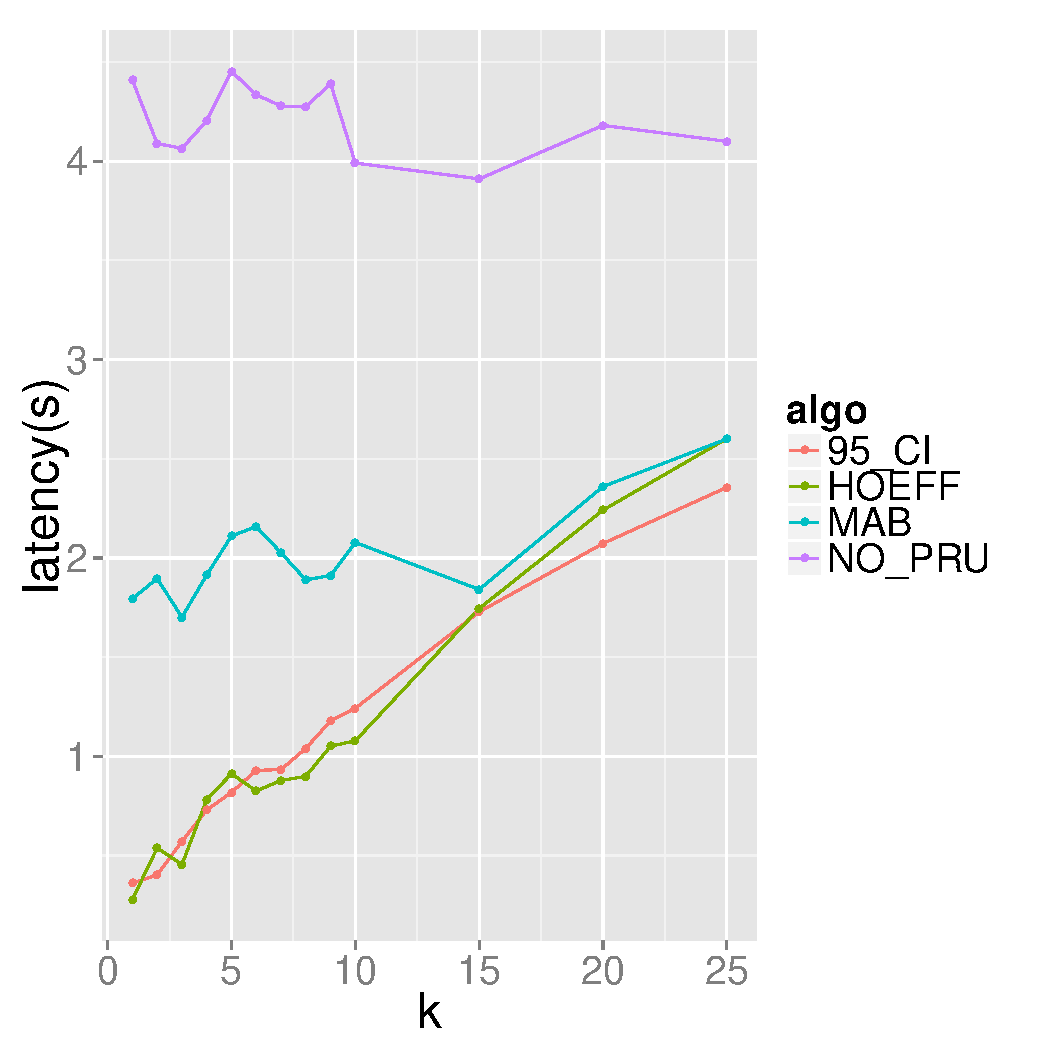
\includegraphics[width=4.2cm] {Images/bank_in_memory_latency.pdf}}
% \caption{Bank dataset: latency}
% \label{fig:bank_latency}
% \end{subfigure}
% \begin{subfigure}{0.49\linewidth}
% \centering
% {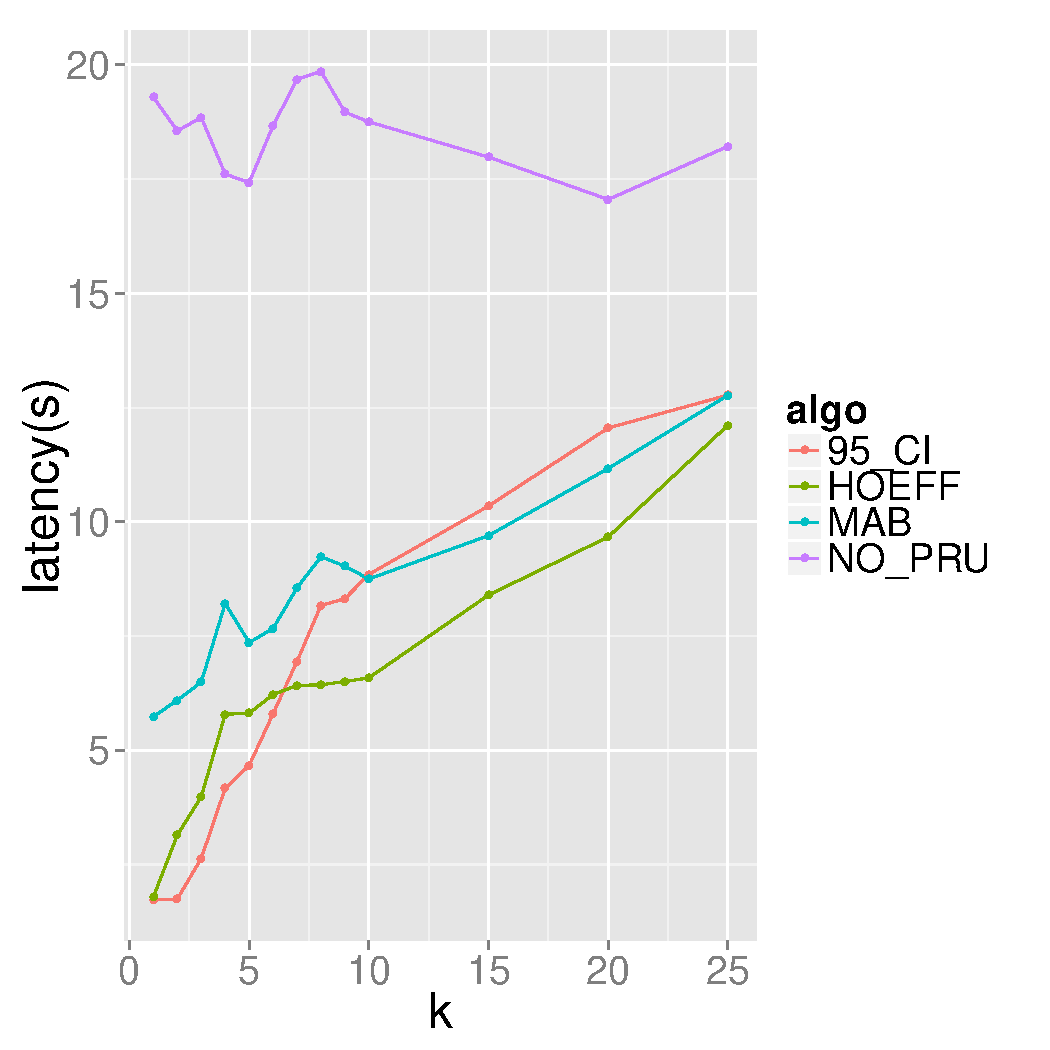
\includegraphics[width=4.2cm] {Images/dia_in_memory_latency.pdf}}
% \caption{Diabetes dataset: latency}
% \label{fig:diabetes_latency}
% \end{subfigure}
% \label{fig:accuracy}
% \caption{Latency for Heuristics}
% \end{figure}

\noindent {\it Accuracy vs. Latency}:
Our MAB and 95\_CI heuristics both have ``knobs'' we can use to study the
tradeoff between accuracy and latency.
In MAB, for example, we can tune the number of phases involved in
processing the entire file. 
Since MAB reduces the number of views by 1 after each phase, the number of
phases is proportional to the pruning power of our algorithm.
A large number of phases means that MAB will prune more views and will prune
them more often.
While this will lead to lower latency, it will also lead to lower accuracy.
Figure \ref{fig:latency_vs_accuracy_mab} shows how latency and accuracy both
reduce as we increase the number of phases in MAB ($k$=15).
Each point on the chart corresponds to a different setting for the number of
phases uses in that implementation of the MAB heuristic.
For 95\_CI, we can vary the $z$-score used
to determine the size of our confidence intervals.
That is, we can decide to take a 50\% confidence interval or a 80\% interval or
a 95\% interval.
If we take a smaller confidence interval, we will have higher pruning and
therefore lower latency.
However, a smaller confidence interval also leads to lower latency since we
prune views with lower confidence.
Figure \ref{fig:latency_vs_accuracy_ci} shows that as the $z$-score of the
confidence interval increases, the accuracy of our heuristics increases, but so
does its latency ($k$=15).
Every point corresponds to a different size of the confidence intervals.

\begin{figure}[h] 
\centering
\begin{subfigure}{0.49\linewidth}
\centering
{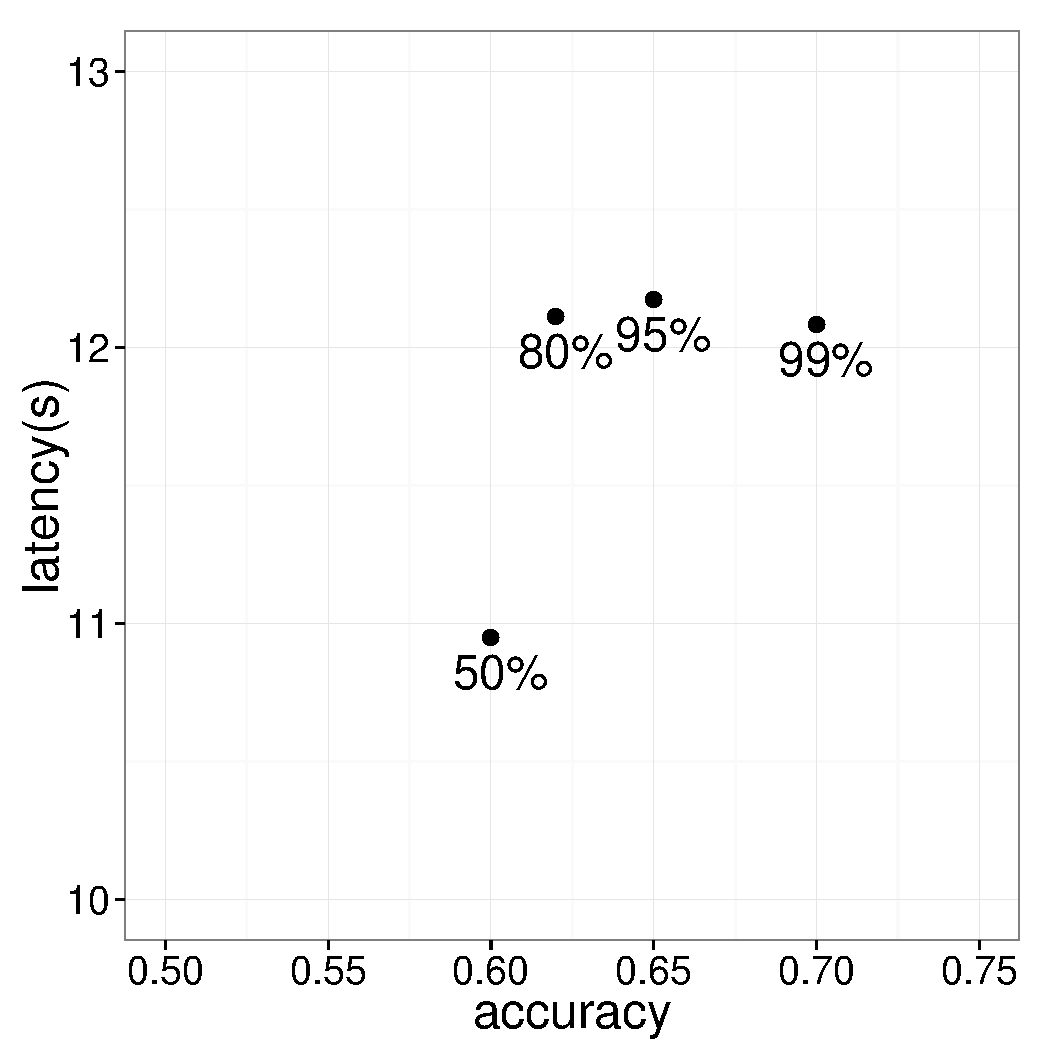
\includegraphics[width=4.2cm] {Images/latency_vs_accuracy_ci.pdf}}
\caption{Latency vs. Accuracy for CI-pruning}
\label{fig:latency_vs_accuracy_ci}
\end{subfigure}
\begin{subfigure}{0.49\linewidth}
\centering
{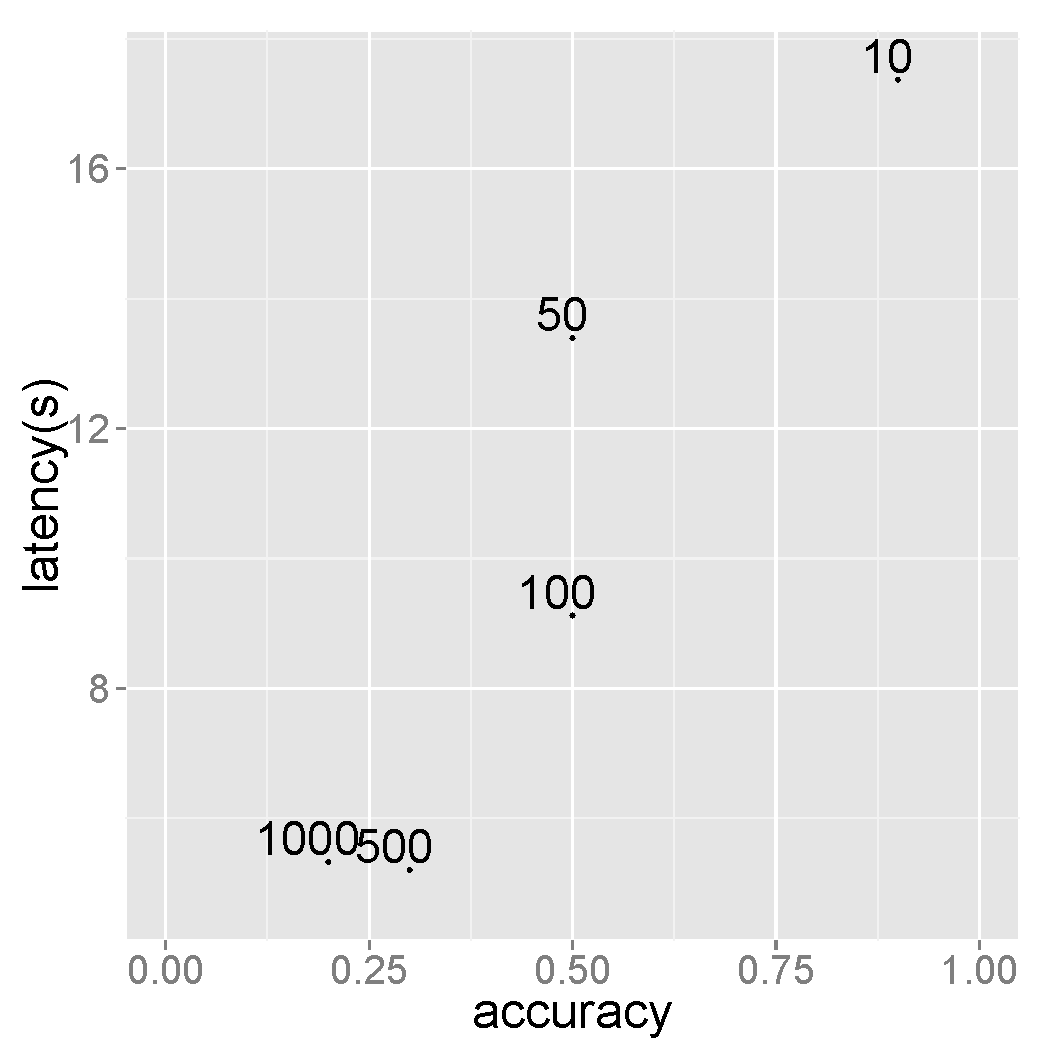
\includegraphics[width=4.2cm] {Images/latency_vs_accuracy_mab.pdf}}
\caption{Latency vs. Accuracy for MAB pruning}
\label{fig:latency_vs_accuracy_mab}
\end{subfigure}
\label{fig:accuracy}
\caption{Latency vs. Accuracy for different heuristics \srm{These plots are very hard to read -- numbers overlap symbols, and symbols are too small.}}
\end{figure}








